% Options for packages loaded elsewhere
\PassOptionsToPackage{unicode}{hyperref}
\PassOptionsToPackage{hyphens}{url}
\PassOptionsToPackage{dvipsnames,svgnames,x11names}{xcolor}
%
\documentclass[
  10pt,
  a4paper,
]{article}
\usepackage{amsmath,amssymb}
\usepackage{iftex}
\ifPDFTeX
  \usepackage[T1]{fontenc}
  \usepackage[utf8]{inputenc}
  \usepackage{textcomp} % provide euro and other symbols
\else % if luatex or xetex
  \usepackage{unicode-math} % this also loads fontspec
  \defaultfontfeatures{Scale=MatchLowercase}
  \defaultfontfeatures[\rmfamily]{Ligatures=TeX,Scale=1}
\fi
\usepackage{lmodern}
\ifPDFTeX\else
  % xetex/luatex font selection
  \setmainfont[AutoFakeBold=2,AutoFakeSlant=0.2]{Noto Sans CJK KR}
  \setsansfont[]{Noto Sans CJK KR}
\fi
% Use upquote if available, for straight quotes in verbatim environments
\IfFileExists{upquote.sty}{\usepackage{upquote}}{}
\IfFileExists{microtype.sty}{% use microtype if available
  \usepackage[]{microtype}
  \UseMicrotypeSet[protrusion]{basicmath} % disable protrusion for tt fonts
}{}
\makeatletter
\@ifundefined{KOMAClassName}{% if non-KOMA class
  \IfFileExists{parskip.sty}{%
    \usepackage{parskip}
  }{% else
    \setlength{\parindent}{0pt}
    \setlength{\parskip}{6pt plus 2pt minus 1pt}}
}{% if KOMA class
  \KOMAoptions{parskip=half}}
\makeatother
\usepackage{xcolor}
\usepackage[margin=23mm]{geometry}
\usepackage{longtable,booktabs,array}
\usepackage{calc} % for calculating minipage widths
% Correct order of tables after \paragraph or \subparagraph
\usepackage{etoolbox}
\makeatletter
\patchcmd\longtable{\par}{\if@noskipsec\mbox{}\fi\par}{}{}
\makeatother
% Allow footnotes in longtable head/foot
\IfFileExists{footnotehyper.sty}{\usepackage{footnotehyper}}{\usepackage{footnote}}
\makesavenoteenv{longtable}
\usepackage{graphicx}
\makeatletter
\def\maxwidth{\ifdim\Gin@nat@width>\linewidth\linewidth\else\Gin@nat@width\fi}
\def\maxheight{\ifdim\Gin@nat@height>\textheight\textheight\else\Gin@nat@height\fi}
\makeatother
% Scale images if necessary, so that they will not overflow the page
% margins by default, and it is still possible to overwrite the defaults
% using explicit options in \includegraphics[width, height, ...]{}
\setkeys{Gin}{width=\maxwidth,height=\maxheight,keepaspectratio}
% Set default figure placement to htbp
\makeatletter
\def\fps@figure{htbp}
\makeatother
\setlength{\emergencystretch}{3em} % prevent overfull lines
\providecommand{\tightlist}{%
  \setlength{\itemsep}{0pt}\setlength{\parskip}{0pt}}
\setcounter{secnumdepth}{5}
\ifLuaTeX
\usepackage[bidi=basic]{babel}
\else
\usepackage[bidi=default]{babel}
\fi
\babelprovide[main,import]{korean}
\ifPDFTeX
\else
\babelfont{rm}[AutoFakeBold=2,AutoFakeSlant=0.2]{Noto Sans CJK KR}
\fi
% get rid of language-specific shorthands (see #6817):
\let\LanguageShortHands\languageshorthands
\def\languageshorthands#1{}
\usepackage{fontspec}
\XeTeXlinebreaklocale "ko"
\XeTeXlinebreakskip = 0pt plus 1pt
\usepackage{fancyhdr}
\pagestyle{fancy}
\fancyhf{}
\fancyhead[L]{\small VigilODE: numerical methods and independent audit}
\fancyfoot[C]{\thepage}
\setlength{\headheight}{14pt}
\setlength{\emergencystretch}{3em}
\AtBeginDocument{\hypersetup{colorlinks=true,linkcolor=blue!45!black,urlcolor=blue!45!black}}
\setcounter{tocdepth}{2}
\ifLuaTeX
  \usepackage{selnolig}  % disable illegal ligatures
\fi
\IfFileExists{bookmark.sty}{\usepackage{bookmark}}{\usepackage{hyperref}}
\IfFileExists{xurl.sty}{\usepackage{xurl}}{} % add URL line breaks if available
\urlstyle{same}
\hypersetup{
  pdftitle={VigilODE: 구조를 보존하는 Rosenbrock 시간 적분과 복사 수송 응용},
  pdflang={ko-KR},
  colorlinks=true,
  linkcolor={Maroon},
  filecolor={Maroon},
  citecolor={Blue},
  urlcolor={Blue},
  pdfcreator={LaTeX via pandoc}}

\title{VigilODE: 구조를 보존하는 Rosenbrock 시간 적분과 복사 수송 응용}
\usepackage{etoolbox}
\makeatletter
\providecommand{\subtitle}[1]{% add subtitle to \maketitle
  \apptocmd{\@title}{\par {\large #1 \par}}{}{}
}
\makeatother
\subtitle{수학적 구성, 구현 사양, 정확도별 계산 비용 및 운영 적합성에
관한 연구보고서}
\author{}
\date{2026년 10월 22일}

\begin{document}
\maketitle

{
\hypersetup{linkcolor=}
\setcounter{tocdepth}{3}
\tableofcontents
}
\hypertarget{uxcd08uxb85d}{%
\section*{초록}\label{uxcd08uxb85d}}
\addcontentsline{toc}{section}{초록}

VigilODE는 강성이 큰 상미분방정식과 공간 이산화된 수송 방정식에 RODAS5P
시간 적분을 적용하는 Rust 수치해석 소프트웨어이다. 연구의 출발점은 고차
시간 적분 자체보다 그 내부 선형계의 표현과 오차의 해석이 실제 계산
비용을 결정한다는 관찰이다. 동일한 시간 적분식을 사용하더라도 모든
상호작용을 조밀 행렬로 구성하면 물리적으로 국소적인 수송과 소수 모멘트에
의한 전역 결합의 구조를 잃는다. 반대로 구조만 강조하고 오차
제어·보간·좌표 복원·실패 처리의 의미를 바꾸면 빠른 계산을 얻어도 원래
문제의 정확도를 보장할 수 없다.

본 보고서는 범용 VigilODE 개발 결과와 비등방 우주론의 광자 수송을 위한
응용 개발 결과를 함께 검토한다. 현재 구현은 여덟 단계 Rosenbrock 적분,
조밀·대역·행렬 없는 선형계 처리, 연속 출력, 제한된 사건 검출, 사용자
정의 단계 선형해법, 그리고 수락된 시간 단계 사이의 보존형 재격자화를
포함한다. 축대칭 광자 수송에서는 각 에너지 군의 삼중대각 행렬과 랭크 2
Thomson 이득항을 분리한다. 에너지 이동 방향이 일관된 경우 이 구성은 단계
선형계의 계산량을 전체 셀 수에 비례하도록 낮춘다. 본문은 이러한 복잡도
감소의 조건, 저랭크 경계 결합의 Schur 소거, 원래 차원을 유지하는 저랭크
보정, 보존형 재매핑의 안정성, 아핀 좌표 축소 후 오차 노름의 복원을
명시적으로 유도한다.

최근 NCP 실행의 게시 자료에는 허용오차 사다리에서 정상 종료한 측정
1,144개, 시간 제한에 도달한 측정 2개, 적용 대상에서 제외된 항목 66개가
포함된다. 미리 정한 상대허용오차 \(10^{-8}\)에서 확인한 VigilODE의 22개
문제·선형해법 조합은 선정된 관측량의 오차 예산 \(10^{-6}\)을 만족하였다.
가장 큰 게시 오차는 약 \(1.23\times10^{-8}\)이다. 구조를 이용한 직접
해법은 시험한 강성 수송 문제에서 유리하였으나, 비강성 문제에서는 Julia와
diffsol의 명시적 방법이 더 빨랐다. 이 결과는 응용별 방법 선택의
근거이다. 전체 분포함수의 오차, 연속체 해의 정확도 또는 임의 문제에 대한
속도 우위를 뜻하지 않는다.

현재 소프트웨어는 검증된 문제에 제한한 연구 계산에 사용할 수 있는 단계에
도달하였다. 범용 production solver로서의 승격에는 전체 상태·공간
분해능·재격자화 오차의 통합 검증, 실제 물리 모델과의 결합, 재현 가능한
원자료 공개, 그리고 변경된 코드의 목표 환경 회귀 실행이 더 필요하다. 본
보고서는 이 구분을 유지하면서, 실제 구현 가능한 후속 작업과 그 완료
조건을 제시한다.

\textbf{주제어:} 강성 상미분방정식, Rosenbrock 방법, 유한체적법, 저랭크
보정, Schur 보완행렬, 복사 수송, 수치 오차 제어.

\hypertarget{uxc5f0uxad6c-uxb3d9uxae30uxc640-uxacc4uxc0b0uxc0c1uxc758-uxc9c8uxbb38}{%
\section{연구 동기와 계산상의
질문}\label{uxc5f0uxad6c-uxb3d9uxae30uxc640-uxacc4uxc0b0uxc0c1uxc758-uxc9c8uxbb38}}

\hypertarget{uxace0uxcc28-uxc801uxbd84uxae30uxc640-uxacc4uxc0b0-uxbe44uxc6a9-uxc0acuxc774uxc758-uxac04uxadf9}{%
\subsection{고차 적분기와 계산 비용 사이의
간극}\label{uxace0uxcc28-uxc801uxbd84uxae30uxc640-uxacc4uxc0b0-uxbe44uxc6a9-uxc0acuxc774uxc758-uxac04uxadf9}}

강성 문제에서 명시적 시간 적분의 단계 크기는 정확도보다 안정성에 의해
제한될 수 있다. 음적 방법은 이 제약을 완화하지만, 각 단계의 선형계 또는
비선형계 해법에 상당한 비용을 지불한다. 따라서 적분기의 형식적 차수만
비교하여 전체 계산의 효율을 예측하기 어렵다. 우변 평가, Jacobian 구성,
행렬 분해, 선형 반복, 오차 추정, 출력 보간과 메모리 관리가 모두 측정
대상이다.

VigilODE의 기본 선택은 RODAS5P이다. 이 방법은 고전적 5(4)차
Rosenbrock--Wanner 구성으로, 매 시간 단계의 선형화 지점에서 만든 하나의
Jacobian을 여러 내부 단계에서 사용한다 {[}7{]}. 이를 통해 비선형 Newton
반복을 내부 단계마다 완결하는 비용을 피하면서 고차 근사를 구성한다. 본
연구의 독자적 관심은 기존 방법의 계수를 새로 발명하는 데 있지 않다.
동일한 적분식과 오차 의미를 유지한 채, 문제의 구조를 선형대수와 자료
배치에 전달하여 실제 계산량을 줄이는 데 있다.

이 목표는 세 질문으로 구체화된다. 첫째, 조밀 행렬의 계산을 어느 조건에서
대역 또는 저랭크 계산으로 정확하게 대체할 수 있는가. 둘째, 그 대체가
실패하거나 적용 조건이 깨질 때 코드가 과거 인수분해나 불완전한 결과를
잘못 재사용하지 않는가. 셋째, 관측량과 전체 상태, 시간 이산화와 공간
이산화의 오차를 구분한 동일한 정확도 조건에서 속도를 비교했는가. 본
보고서의 수학, 코드 검토와 실험 해석은 이 세 질문에 대응한다.

\hypertarget{uxc18cuxcc28uxc6d0-uxbc18uxc751uxb9dduxc5d0uxc11c-uxc704uxc0c1uxacf5uxac04-uxc218uxc1a1uxc73cuxb85c}{%
\subsection{소차원 반응망에서 위상공간
수송으로}\label{uxc18cuxcc28uxc6d0-uxbc18uxc751uxb9dduxc5d0uxc11c-uxc704uxc0c1uxacf5uxac04-uxc218uxc1a1uxc73cuxb85c}}

복사와 물질이 결합된 우주론 계산에서 광자를 소수의 모멘트로 닫을 수
있다면 상태 차원은 작다. 그러나 에너지와 방향에 의존하는 분포함수
\(f(E,\hat e,t)\)를 직접 풀면 상태 수는 에너지 셀 수와 각도 셀 수의
곱으로 증가한다. 축대칭에서는 \(N_E N_\mu\), 일반적인 방향 의존성에서는
\(N_E N_\mu N_\phi\)에 물질·기하 변수와 보존량 기록 변수가 더해진다.
이때 조밀 LU 분해의 \(O(N^3)\) 비용은 고차 적분기의 장점을 쉽게
압도한다.

물리적 결합은 그보다 단순한 구조를 가진다. 에너지·각도 이류는 인접 셀을
연결한다. 냉각된 전자의 비편광 Thomson 산란은 각도 전체를 연결하지만,
이득항은 소수의 각도 모멘트로 표현된다. 물질의 온도·이온화율·비등방
응력은 많은 광자 셀과 연결되지만 변수의 개수는 상대적으로 작다. 이
구조는 대역 행렬, 에너지 블록별 저랭크 보정, 작은 경계 블록의 Schur
소거를 자연스럽게 만든다.

이러한 구성은 특정 물리 조건 아래 정확한 선형대수 알고리즘이다. 반복
수가 항상 일정하리라는 경험적 기대와 구분해야 한다. 단방향 에너지
이류에서는 블록 삼각 소거를 사용할 수 있지만, 방향에 따라 에너지 이류의
부호가 달라지면 그 순서가 사라진다. 후자의 경우 반복 해법과 전처리의
수렴을 따로 평가해야 한다.

\hypertarget{uxac80uxd1a0-uxb300uxc0c1uxacfc-uxc99duxac70uxc758-uxbc94uxc704}{%
\subsection{검토 대상과 증거의
범위}\label{uxac80uxd1a0-uxb300uxc0c1uxacfc-uxc99duxac70uxc758-uxbc94uxc704}}

소스 검토의 기준은 2026년 10월 22일에 확인한 저장소의
\texttt{555e71e03fe31e6c9b21961c8e2d263b1794eb6f} 상태이다. 이 상태는
VigilODE 자체의 범용 개발 결과를 이미 포함한다. 별도 연구 브랜치의 아핀
축소 오차 노름과 별도 결과 브랜치의 측정 자료도 통합 검토하였다. 최근
물리 응용만으로 범용 기능을 대표시키거나, 오래된 결과를 최신 코드의 직접
실행 결과로 간주하지 않았다.

이 문서는 소스에서 확인한 기능, 수학적 명제, 게시된 수치 결과 및 이번
검토에서 추가한 구현을 서로 구분한다. 과거에 게시되어 전제가 유지된
결과는 다시 실행하여 새로운 결과처럼 세지 않았다. 새 수정의 표적 회귀
검사는 별도 검증 기록으로 제공한다. 본 보고서는 외부 심사를 위해 작성된
기술 문서이며, 사람 심사자의 독립적인 승인이나 학술지 게재를 뜻하지
않는다.

\hypertarget{uxc218uxd559uxc801-uxbb38uxc81cuxc640-uxc624uxcc28uxc758-uxc758uxbbf8}{%
\section{수학적 문제와 오차의
의미}\label{uxc218uxd559uxc801-uxbb38uxc81cuxc640-uxc624uxcc28uxc758-uxc758uxbbf8}}

\hypertarget{uxc2dcuxac04-uxc801uxbd84-uxbb38uxc81c}{%
\subsection{시간 적분
문제}\label{uxc2dcuxac04-uxc801uxbd84-uxbb38uxc81c}}

기본 문제는

\[
\dot y(t)=f(t,y(t)),\qquad y(t_0)=y_0,\qquad y\in\mathbb R^N
\]

이다. 제한된 경로에서는 상수 질량행렬 \(M\)을 갖는 \(M\dot y=f(t,y)\)도
지원하며, 특이 질량행렬을 이용한 지수 1 미분대수방정식은 해당 해법의
일관성 조건 아래에서 다룬다. 임의의 상태 의존 질량행렬 또는 임의 지수의
미분대수방정식을 지원한다는 의미는 아니다.

우변과 Jacobian의 매끄러움, 해의 존재 구간, 시간 단계와 공간 이산화의
관계는 문제에 따라 별도로 주어진다. 고전적인 차수 조건은 충분한
매끄러움을 전제로 한다. 이온화 문턱의 통과, 제한자의 분기, 재격자화 또는
강성 극한에서는 이 전제를 다시 확인해야 한다. 특히 공간 이산화로 얻은
강성 계열에서 고전적 차수가 그대로 관측되리라는 보장은 없다. Rosenbrock
방법의 편미분방정식 적용에서 이 구분은 알려진 중요 문제이다 {[}2{]}.

\hypertarget{uxad6duxc18c-uxc624uxcc28-uxc2dcuxd5d8uxacfc-uxc804uxc5ed-uxc624uxcc28}{%
\subsection{국소 오차 시험과 전역
오차}\label{uxad6duxc18c-uxc624uxcc28-uxc2dcuxd5d8uxacfc-uxc804uxc5ed-uxc624uxcc28}}

성분별 허용 척도를

\[
s_i=\operatorname{atol}_i+\operatorname{rtol}\max(|y_{n,i}|,|y_{n+1,i}|)
\]

로 정의하고, 국소 오차 추정 벡터 \(e\)에 대해

\[
\|e\|_{\mathrm{WRMS}}=
\left[\frac1N\sum_{i=1}^N\left(\frac{e_i}{s_i}\right)^2\right]^{1/2}
\]

를 사용한다. 이것은 단계 수락을 위한 추정량이다. 누적 전역 오차의
상한이나 모든 성분의 최대 오차가 아니다. 하나의 성분만 오차를 가지면
WRMS에서 \(1/\sqrt N\) 인자가 적용된다. 따라서 물리적으로 중요한 소수
변수의 정확도를 지키려면 그 변수의 허용 척도와 출력 검사를 명시해야
한다.

영인 척도도 해석이 필요하다. 해당 성분의 추정 오차가 함께 영이면 기여를
영으로 둘 수 있지만, 척도는 영이고 오차가 영이 아니면 단계는 거절되어야
한다. NaN이나 무한대가 작게 보이도록 비교 연산을 구성해서는 안 된다.
현재 구현은 비유한 단계 결과를 실패로 처리하고, 지원되지 않는 허용오차
조합을 묵시적으로 스칼라로 바꾸지 않고 거절한다.

관측량 오차는 별도이다. 예를 들어 광자 수와 복사 에너지가 정확하더라도
각도 분포의 고차 성분이 잘못될 수 있다. 한편 전체 상태의 단순 상대오차는
물리적으로 소멸하는 성분을 과도하게 강조할 수 있다. 따라서 전체 상태,
중요 관측량, 보존량 및 근영점 성분을 병렬로 평가하는 것이 적절하다. 어느
하나를 다른 하나의 증거로 대체하지 않는다.

\hypertarget{rodas5puxc758-uxc2e4uxc81c-uxacc4uxc0b0uxc2dduxacfc-uxad6cuxd604-uxc0acuxc591}{%
\section{RODAS5P의 실제 계산식과 구현
사양}\label{rodas5puxc758-uxc2e4uxc81c-uxacc4uxc0b0uxc2dduxacfc-uxad6cuxd604-uxc0acuxc591}}

\hypertarget{uxc5ecuxb35f-uxb2e8uxacc4uxc640-uxacf5uxd1b5-uxb2e8uxacc4-uxd589uxb82c}{%
\subsection{여덟 단계와 공통 단계
행렬}\label{uxc5ecuxb35f-uxb2e8uxacc4uxc640-uxacf5uxd1b5-uxb2e8uxacc4-uxd589uxb82c}}

현재 계수 스냅샷의 단계 수는 여덟이다. 대각 계수는
\(\gamma=0.21193756319429014\)이다. 계수는 SciML의 공개 RODAS5P 표에서
가져온 십진 리터럴이며, 원래의 정확한 유리수나 임의 정밀도 계수로
취급하지 않는다 {[}1{]}. 스냅샷의 SHA-256을 검사한 뒤 프로세스 수명 동안
한 번 파싱하여 재사용한다.

빠른 경로는 변환된 단계 변수 \(u_i\)를 사용한다.
\(J_n=\partial_y f(t_n,y_n)\), \(f_{t,n}=\partial_t f(t_n,y_n)\)이고
\(h\)가 시도할 시간 단계이면,

\[
W_n=\frac{1}{h\gamma}I-J_n,
\]

\[
W_nu_i=f\!\left(t_n+c_ih,\ y_n+\sum_{j<i}a_{ij}u_j\right)
 +\frac1h\sum_{j<i}C_{ij}u_j+h\gamma_i f_{t,n},
\qquad i=1,\ldots,8.
\]

여기서 \(\gamma_i\)는 저장된 변환 계수 행렬의 해당 행 합이다. 해와 내장
오차 추정치는

\[
y_{n+1}=y_n+\sum_{i=1}^8b_i^{\mathrm{code}}u_i,
\qquad e_n=u_8
\]

로 계산한다. 첫 단계의 우변은 이미 계산한 \(f(t_n,y_n)\)를 사용한다.
이후 단계에서는 실제 단계 상태에서 우변을 다시 평가한다. 따라서 한
단계에서 Jacobian을 고정한다는 사실은 비선형 우변 자체를 고정한다는 뜻이
아니다.

이 표현은 동일한 방법을 계산하면서 단계마다 추가 Jacobian 곱을 구성하지
않게 한다. 한 번의 시도에서 \(W_n\)은 공통이므로 직접 해법은 한 번
인수분해한 뒤 여덟 번 삼각계 풀이를 수행한다. 국소 오차로 거절된
재시도는 수락 상태가 같으므로 해당 위치의 Jacobian, 초기 우변과 시간
편미분을 재사용할 수 있으나, 바뀐 \(h\)에 맞는 단계 행렬의 준비는 다시
필요하다. 함수 평가나 선형해법 자체가 실패한 경우에는 실패 원인에 맞게
재선형화한다.

\hypertarget{uxc2e4uxd589-uxc21cuxc11c}{%
\subsection{실행 순서}\label{uxc2e4uxd589-uxc21cuxc11c}}

한 번의 수락 단계는 다음과 같이 구성된다.

\begin{enumerate}
\def\labelenumi{\arabic{enumi}.}
\tightlist
\item
  입력 차원, 허용오차, 시간 구간과 지원 조합을 검사하고 적분 작업공간을
  준비한다.
\item
  현재 수락 상태에서 우변, 필요한 시간 편미분 및 Jacobian 또는 사용자
  정의 선형화 자료를 계산한다.
\item
  제안된 \(h\)에서 단계 행렬을 준비한다. 수치적으로 무효한 인수분해는
  사용할 수 있는 상태로 남겨 두지 않는다.
\item
  여덟 단계의 우변과 선형계를 순서대로 계산하고, 새 상태와 내장 오차를
  만든다.
\item
  국소 오차, 비유한 값, 선택된 내부 출력 오차 추정과 실패 종류를
  평가한다.
\item
  수락한 경우에만 시간과 상태를 변경한다. 출력과 사건 위치는 지정한
  경로의 의미에 따라 처리한다.
\item
  재격자화가 요청되면 수락된 상태에서 별도의 후보를 만들고, 새
  격자·상태·선형계 자료의 유효성을 확인한 뒤 교체한다.
\end{enumerate}

이 순서에서 선형계 성공과 시간 단계 성공은 다르다. 작은 선형 잔차는 단계
방정식을 잘 풀었다는 뜻이고, 시간 적분 오차가 작다는 결론에는
우변·계수·단계 구성·오차 추정의 정합성이 추가로 필요하다.

\hypertarget{uxc8fcuxc694-uxc0acuxc591}{%
\subsection{주요 사양}\label{uxc8fcuxc694-uxc0acuxc591}}

\begin{longtable}[]{@{}
  >{\raggedright\arraybackslash}p{(\columnwidth - 2\tabcolsep) * \real{0.5000}}
  >{\raggedright\arraybackslash}p{(\columnwidth - 2\tabcolsep) * \real{0.5000}}@{}}
\toprule\noalign{}
\begin{minipage}[b]{\linewidth}\raggedright
항목
\end{minipage} & \begin{minipage}[b]{\linewidth}\raggedright
확인한 구현과 의미
\end{minipage} \\
\midrule\noalign{}
\endhead
\bottomrule\noalign{}
\endlastfoot
언어·산술 & Rust 2024 edition, 최소 Rust 1.94.1, 주요 수치 경로는
binary64 \\
기본 방법 & 여덟 단계 RODAS5P, 공통 Jacobian, 적응형 시간 단계 \\
기본 허용오차 & \texttt{rtol=1e-6}, \texttt{atol=1e-9}; 문제별 재설정
필요 \\
초기 단계·최대 시도 & 기본 \texttt{h0=1e-3}, 최대 시도 100,000; 수락과
거절을 함께 셈 \\
우변 공급 & 메모리를 미리 제공하는 콜백, 자율계 선언, 시간 편미분
공급 \\
Jacobian 공급 & 조밀, 대역, 유한차분, Jacobian-벡터 곱 \\
직접 선형해법 & 조밀 LU, 대역 LU; 크기와 경로에 따라 구현 선택 \\
반복 선형해법 & 행렬 없는 GMRES 계열; 전처리와 실제 잔차 확인 \\
허용오차 벡터 & 조밀·대역 빠른 경로에서 지원; 일부 질량행렬·행렬 없는
조합은 거절 \\
연속 출력 & RODAS5P 연속 확장; 내부 오차 추정을 켜거나 끌 수 있음 \\
내부 오차 추정 & 기본은 해당 단계 행렬로 거른 중점 결함 추정; 엄밀한
상계가 아님 \\
질량행렬 & 제한된 순차 조밀 경로; 성능·기능 제약을 별도 확인해야 함 \\
사건 검출 & 연속 확장의 부호 변화를 이용한 후처리; 접선 접촉과 다중
교차를 놓칠 수 있음 \\
종료 사건 & 현재는 계산 후 출력을 잘라내며, 사건 이후 계산을 즉시
중단하지 않음 \\
응용 선형계 & 사용자 정의 단계 선형화·인수분해·풀이 인터페이스 \\
재격자화 & 수락 단계 사이의 보존형 매핑, 모델 및 선형계 재결합, 분할
적분 \\
\end{longtable}

표의 기능은 모두 같은 실행 경로에서 동시에 사용할 수 있는 선택지가
아니다. 예를 들어 Jacobian-벡터 곱만 제공하는 문제에서 연속 출력이나
질량행렬을 요청하면 지원되지 않는 조합으로 처리한다. 공개 인터페이스의
성능 선택 모드 역시 현재 별도 가속 후보로 자동 전환하지 않고 기본적으로
같은 검증된 기본 수치 경로를 실행한다. 이름에 근거해 기능이나 속도
차이를 추정해서는 안 된다.

\hypertarget{uxbcf4uxc874uxd615-uxbcf5uxc0ac-uxc218uxc1a1uxacfc-uxacf5uxac04-uxc774uxc0b0uxd654}{%
\section{보존형 복사 수송과 공간
이산화}\label{uxbcf4uxc874uxd615-uxbcf5uxc0ac-uxc218uxc1a1uxacfc-uxacf5uxac04-uxc774uxc0b0uxd654}}

\hypertarget{uxbb3cuxb9ac-uxbcc0uxc218uxc640-uxc88cuxd45c}{%
\subsection{물리 변수와
좌표}\label{uxbb3cuxb9ac-uxbcc0uxc218uxc640-uxc88cuxd45c}}

본 응용의 기본 물리 범위는 기울어지지 않은 Bianchi I 배경에서의 스칼라
비편광 광자이다. 계량 부호는 \((-,+,+,+)\), 시간은 고유시간, \(E\)는
광자 에너지이며 \(c\)와 \(\hbar\)를 유지한다. 편광 상태 하나당 점유수
\(f\)에 대해

\[
\kappa=\frac{g}{(2\pi\hbar)^3c^3},\qquad
n_\gamma=\kappa\int E^3f\,dq\,d\Omega,
\qquad
\rho_\gamma=\kappa\int E^4f\,dq\,d\Omega,
\quad q=\log(E/E_{\rm ref})
\]

이다. 비편광 두 자유도를 따로 합하지 않은 \(f\)에는 \(g=2\)를 쓴다. 이미
합해진 분포에 다시 \(g\)를 곱해서는 안 된다. 코드의 광자 셀 변수는
\(f\)의 무가중 평균이 아니라 적절한 위상공간 측도가 포함된 셀 적분이다.

평균 팽창률 \(H=\dot a/a\)와 무추적 전단 \(\sigma_{ab}\)에 대해 광선의
운동은

\[
\dot q=-H-S(\hat e),\qquad
\dot e^a=-\sigma^a{}_be^b+S(\hat e)e^a,
\qquad S(\hat e)=\sigma_{ab}e^ae^b
\]

이다. \(e_a\dot e^a=0\)이므로 방향 운동은 구면에 접한다. 축대칭 전단
\(\sigma=\operatorname{diag}(-s,-s,2s)\)과 \(\mu=\cos\theta\)에서는

\[
v_q=-H-s(3\mu^2-1),\qquad
v_\mu=-3s\mu(1-\mu^2).
\]

공변 에너지 좌표 \(x=\log(aE/E_{\rm ref})\)로 바꾸면 등방 팽창항은
제거되지만 전단에 의한 이동은 남는다. 물리 에너지에 고정된 이온화 문턱은
\(x\)에서 이동한다. 따라서 공변 좌표를 사용한다고 흡수 계수가 시간
독립적으로 바뀌는 것은 아니다.

\hypertarget{uxc815uxb9ac-1-uxbcf4uxc874-uxbcc0uxc218uxc758-uxad6cuxc131}{%
\subsection{정리 1: 보존 변수의
구성}\label{uxc815uxb9ac-1-uxbcf4uxc874-uxbcc0uxc218uxc758-uxad6cuxc131}}

\textbf{명제.} 위 Bianchi I 조건에서 \(U=a^3\kappa E^3f\)는

\[
\partial_tU+\partial_q(v_qU)+\nabla_{S^2}\cdot(v_\Omega U)
 =a^3\kappa E^3 C_t[f]
\]

를 만족한다. 여기서 \(C_t\)는 고유시간당 충돌항이다.

\textbf{증명.} \(S\)는 무추적 이차식이므로 구면의 \(\ell=2\)
조화함수이며 \(\Delta_{S^2}S=-6S\)이다. 방향 속도는
\(v_\Omega=-\frac12\nabla_{S^2}S\)이므로
\(\nabla_{S^2}\cdot v_\Omega=3S\)이다. 또한 \(v_q=-H-S\)이고 \(q\)에
독립적이므로

\[
3H+3v_q+\partial_qv_q+\nabla_{S^2}\cdot v_\Omega
 =3H-3H-3S+3S=0.
\]

수송 방정식
\(\partial_tf+v_q\partial_qf+v_\Omega\cdot\nabla f=C_t[f]\)에
\(a^3\kappa E^3\)을 곱하고 곱의 미분을 전개하면, 위 항등식에 의해 추가
부피 변화항이 상쇄된다. 따라서 보존형 식을 얻는다. \(\square\)

축대칭이면 \(d\Omega=2\pi\,d\mu\)이고 셀 내용은

\[
N_{ij}=\int_{q_{i-1/2}}^{q_{i+1/2}}
       \int_{\mu_{j-1/2}}^{\mu_{j+1/2}}2\pi U\,d\mu\,dq
\]

이다. 이 정의는 광자 수 보존을 직접 검사하게 한다. 일반적인 방향
의존성을 한 각도만으로 표현하려면 축대칭이라는 추가 가정이 필요하다.
현재의 응용 구현은 VigilODE 저장소 안의 실행 가능한 고객 모형이며 실제
BASS/rei 전체 계산에 이미 연결되었다는 의미는 아니다. 전체 구면 모형은
두 각도 좌표를 사용하지만, 일반 Bianchi 기하·기울기·편광을 모두 포함하는
완결된 Einstein--Boltzmann 모형으로 해석하지 않는다.

\hypertarget{uxc720uxd55cuxccb4uxc801-uxc5f0uxc0b0uxc790uxc640-uxbcf4uxc874uxb7c9}{%
\subsection{유한체적 연산자와
보존량}\label{uxc720uxd55cuxccb4uxc801-uxc5f0uxc0b0uxc790uxc640-uxbcf4uxc874uxb7c9}}

현재 수송 이산화는 비균일 격자에서의 일차 upwind 유한체적법이다. 한 내부
면의 플럭스를 한 번 계산하여 두 인접 셀에 서로 반대 부호로 더한다.
따라서 내부 플럭스의 총합은 대수적으로 상쇄된다. 에너지 경계의 유출은
별도 누적 변수에 기록하고, 흡수된 광자 역시 소거하지 않고 해당 반응 기록
변수에 더한다. 광자 셀과 이 기록 변수의 합은 반이산 방정식의 선형
불변량이다.

축대칭 모형의 상태 차원은

\[
N=2+N_q(N_\mu+1)
\]

이다. 양 끝의 두 변수는 경계 유출이며 각 에너지 군에는 \(N_\mu\)개의
광자 셀과 하나의 흡수 기록 변수가 있다. 전체 구면에서는

\[
N=2+N_q(N_\mu N_\phi+1)
\]

로 바뀐다. 물질·전단 결합은 추가 상태 변수를 사용한다.

공간의 일차 절단오차는 시간 적분을 다섯 차로 수행해도 사라지지 않는다.
고정 격자에서 반이산 기준해에 수렴하는 시험과 격자를 세분하여 연속체
기준해에 수렴하는 시험을 분리해야 한다. 반이산 기준해와의 \(10^{-8}\)
차이가 연속체 해의 \(10^{-8}\) 정확도를 증명하지 않는 이유가 여기에
있다.

\hypertarget{thomson-uxc0b0uxb780uxc758-uxc800uxb7aduxd06c-uxad6cuxc870}{%
\subsection{Thomson 산란의 저랭크
구조}\label{thomson-uxc0b0uxb780uxc758-uxc800uxb7aduxd06c-uxad6cuxc870}}

냉각된 전자의 탄성·비편광 Thomson 산란을 축대칭으로 줄이면

\[
C[f]=\Gamma\left\{\int_{-1}^1
\left[1+\frac12P_2(\mu)P_2(\mu')\right]
f(\mu')\frac{d\mu'}2-f(\mu)\right\},\qquad
\Gamma=c\sigma_Tn_e.
\]

각도 셀 폭 \(d_j=\Delta\mu_j\)와 \(P_2\)의 셀 평균 \(p_j\)에 대해, 한
에너지 군의 이득항은

\[
\dot N_j\big|_{\rm scatt}
=\Gamma\left[\frac{d_j}{2}M_0+\frac{d_jp_j}{4}M_2-N_j\right],
\quad M_0=\sum_jN_j,\quad M_2=\sum_jp_jN_j
\]

이다. 모멘트 두 개를 계산한 뒤 각 셀에 다시 분배하므로 연산량은
\(O(N_\mu)\)이다. 모든 셀 쌍을 직접 연결하는 \(O(N_\mu^2)\) 계산이
필요하지 않다. \(\sum_jd_j=2\)와 \(\sum_jd_jp_j=0\)이므로
\(\sum_j\dot N_j=0\)도 바로 따른다.

이 랭크 2 구조는 \textbf{에너지 군마다} 성립한다. 에너지 군 전체를
하나의 상수 계수 저랭크 행렬로 취급하면 잘못된 복잡도 결론을 얻는다.
일반 구면의 비편광 모형은 단극자 하나와 사중극자 다섯 개로 이득항을
표현하여 군당 랭크 6 표현를 사용한다. 편광과 비탄성 에너지 교환을
포함하면 이 구조와 차원이 달라진다.

\hypertarget{uxad6cuxc870uxb97c-uxc774uxc6a9uxd55c-uxc120uxd615uxacc4-uxd574uxbc95uxacfc-uxbcf5uxc7a1uxb3c4}{%
\section{구조를 이용한 선형계 해법과
복잡도}\label{uxad6cuxc870uxb97c-uxc774uxc6a9uxd55c-uxc120uxd615uxacc4-uxd574uxbc95uxacfc-uxbcf5uxc7a1uxb3c4}}

\hypertarget{uxc5d0uxb108uxc9c0-uxad70uxbcc4-uxc9c1uxc811-uxd480uxc774}{%
\subsection{에너지 군별 직접
풀이}\label{uxc5d0uxb108uxc9c0-uxad70uxbcc4-uxc9c1uxc811-uxd480uxc774}}

한 에너지 군의 단계 행렬을

\[
W_i=H_i-\Gamma U_iV_i^T,\qquad H_i=T_i+\Gamma I,
\quad U_i=\left(\frac d2,\frac{d\circ p}{4}\right),
\quad V_i=(\mathbf1,p)
\]

로 쓴다. \(T_i\)는 각도 이류, 에너지 유출, 흡수 및 시간 이동항을
포함한다. \(H_i\)는 삼중대각이므로 Thomas 소거로 우변과 두 열을 선형
비용에 풀 수 있다. \(y=H_i^{-1}b\), \(Z=H_i^{-1}U_i\), \(m=V_i^Tx\)이면

\[
x=y+\Gamma Zm,\qquad
(I-\Gamma V_i^TZ)m=V_i^Ty.
\]

마지막 식은 \(2\times2\) 선형계이다. 이 작은 행렬이 가역일 때 원래 군의
해를 정확히 구성한다.

에너지 이류가 모든 각도 열에서 같은 방향이면 에너지 군 간 결합은 블록
삼각이 된다. 상류 군부터 위 절차를 적용하여 전체 단계 선형계를 푼다. 각
군의 비용이 \(O(N_\mu)\)이므로 총 비용은 \(O(N_qN_\mu)\)이다. 현재
구현의 명시된 산술 계수에 따르면 군별 인수분해는 \(N_q(29N_\mu-3)\)회,
유출 경계가 있는 정확 풀이 한 번은 \(N_q(15N_\mu+9)+4\)회의 기본
사칙연산을 센다. 이 수에는 기하 계산, 우변 구성, 선형화, 오차 제어와
출력 비용이 포함되지 않는다.

물리 에너지 좌표에서 \(H>2|s|\)는 모든 \(v_q\)가 음수가 되게 하는
충분조건이다. 코드의 실제 적용 여부는 셀별 이류 방향을 확인한다. 공변
좌표나 큰 전단에서는 방향이 섞일 수 있다. 그때 직접 삼각 풀이를 그대로
적용하지 않고 적용 불가를 반환하거나 반복 해법으로 전환해야 한다.

\hypertarget{uxac15uxd55c-uxc0b0uxb780uxc5d0uxc11c-uxc791uxc740-uxd589uxb82cuxc758-uxc0c1uxc1c4-uxd68cuxd53c}{%
\subsection{강한 산란에서 작은 행렬의 상쇄
회피}\label{uxac15uxd55c-uxc0b0uxb780uxc5d0uxc11c-uxc791uxc740-uxd589uxb82cuxc758-uxc0c1uxc1c4-uxd68cuxd53c}}

교과서적인 작은 행렬의 성분 \(1-\Gamma\mathbf1^Tz_1\)은 강한 산란에서
거의 같은 두 수를 뺄 수 있다. 단순한 등방 극한에서는 이 값이
\(\alpha/(\alpha+\Gamma)\) 꼴이고, \(\Gamma\gg\alpha\)이면 상대정확도를
잃기 쉽다. 여기서 \(\alpha\)는 시간 이동 및 흡수·유출의 척도이다.

각도 수송이 수를 보존하므로 \(\mathbf1^TT_i=g^T\)라 하자.
\(H_iz_1=d/2\), \(H_iz_2=(d\circ p)/4\)를 왼쪽에서 \(\mathbf1^T\)로
곱하면

\[
g^Tz_1+\Gamma\mathbf1^Tz_1=\frac12\sum_jd_j,
\quad
g^Tz_2+\Gamma\mathbf1^Tz_2=\frac14\sum_jd_jp_j.
\]

따라서 작은 행렬의 첫째 행을

\[
\left[g^Tz_1+1-\frac12\sum_jd_j\right]m_0
+\left[g^Tz_2-\frac14\sum_jd_jp_j\right]m_2
=\mathbf1^Ty
\]

로 바꿀 수 있다. 이상적인 구적 항등식에서는 보정항이 영이고, 저장된
부동소수점 격자에서는 그 잔차를 보상 합으로 계산한다. \(H_i\)가 해당
수송의 대각우세 M-행렬이고 \(g,d\)가 양수이면 \(g^Tz_1\)은 양수들의
합이다. 이 표현은 작은 양수를 큰 두 수의 차로 만드는 상쇄를 피한다.
행렬의 조건수 자체를 없애는 변환은 아니므로, 잔차와 극한 시험은 여전히
필요하다.

\hypertarget{uxc815uxb9ac-2-uxc791uxc740-uxbb3cuxc9c8-uxacbduxacc4uxc758-schur-uxc18cuxac70}{%
\subsection{정리 2: 작은 물질 경계의 Schur
소거}\label{uxc815uxb9ac-2-uxc791uxc740-uxbb3cuxc9c8-uxacbduxacc4uxc758-schur-uxc18cuxac70}}

Schur 보완행렬을 이용한 블록 해법과 전처리의 수렴 관계는 기존
수치선형대수의 결과이다 {[}3{]}, {[}4{]}. 여기서는 현재 구현에 필요한
식과 복잡도를 직접 전개한다.

\textbf{명제.} 단계 행렬이

\[
\mathcal M=\begin{pmatrix}A&B\\C&D\end{pmatrix},
\qquad A\in\mathbb R^{n\times n},\quad D\in\mathbb R^{m\times m}
\]

이고 \(A\)와 \(S=D-CA^{-1}B\)가 가역이면,
\(\mathcal M(u,v)^T=(f,g)^T\)의 해는

\[
w=A^{-1}f,\qquad Z=A^{-1}B,
\qquad v=S^{-1}(g-Cw),\qquad u=w-Zv
\]

이다.

\textbf{증명.} 첫째 블록 식은 \(u=A^{-1}(f-Bv)=w-Zv\)를 준다. 이를 둘째
식에 대입하면 \(Cw+(D-CZ)v=g\)이므로 위 \(v\)를 얻는다. 다시 첫째 식에
대입하면 유일한 \(u\)가 정해진다. 두 블록 식을 만족하고 가역성을
가정했으므로 해는 유일하다. \(\square\)

\(A\)의 대역폭을 \(b\)라 하고 대역 분해 비용이 \(O(nb^2)\), 한 번의
풀이가 \(O(nb)\)라고 하자. 준비 비용은

\[
O(nb^2+nbm+nm^2+m^3)
\]

이고, 새 우변 하나의 비용은

\[
O(nb+nm+m^2)
\]

이다. \(b,m\)이 고정되어야 \(n\)에 대해 선형이라고 말할 수 있다. 다차원
격자의 자연 순서에서 대역폭이 격자 크기와 함께 커지는 경우에는 이 조건을
충족하지 않는다. 축대칭 에너지 군 해법은 전체 대역폭에 의존하는 소거
대신 군별 구조를 사용하여 이 문제를 피한다.

\hypertarget{uxc815uxb9ac-3-uxc6d0uxb798-uxcc28uxc6d0uxc744-uxc720uxc9c0uxd558uxb294-uxc800uxb7aduxd06c-uxbcf4uxc815}{%
\subsection{정리 3: 원래 차원을 유지하는 저랭크
보정}\label{uxc815uxb9ac-3-uxc6d0uxb798-uxcc28uxc6d0uxc744-uxc720uxc9c0uxd558uxb294-uxc800uxb7aduxd06c-uxbcf4uxc815}}

작은 물질 경계 외에 \(A+UV^T\) 형태의 추가 전역 결합이 있다고 하자.
\(U,V\in\mathbb R^{n\times r}\)이고

\[
\mathcal M_r=\begin{pmatrix}A+UV^T&B\\C&D\end{pmatrix}.
\]

보조 변수 \(z=V^Tu\)를 도입하여

\[
\widehat{\mathcal M}=
\begin{pmatrix}A&B&U\\C&D&0\\-V^T&0&I_r\end{pmatrix}
\]

를 구성한다. 다음 결과는 원래 반복 공간의 차원을 늘리지 않고 이 구성을
사용하는 근거이다.

\textbf{명제.} \(E(f,g)=(f,g,0)\), \(R(u,v,z)=(u,v)\)라 하자. 두 행렬이
가역이면

\[
\mathcal M_r^{-1}=R\widehat{\mathcal M}^{-1}E.
\]

\textbf{증명.} 확대계의 마지막 행은 \(z=V^Tu\)이다. 이를 첫째 행에
대입하면 \((A+UV^T)u+Bv=f\)가 되고, 둘째 행은 \(Cu+Dv=g\)이다. 따라서
확대계의 해를 제한한 벡터는 원래 계의 유일해이다. 모든 우변에 대해
성립하므로 역행렬 항등식을 얻는다. \(\square\)

준비할 작은 경계의 크기는 \(m+r\)이다. 그러므로 위 Schur 복잡도에서
\(m\)을 \(m+r\)로 바꾸면 된다. 대수적 정리는 가역성을 가정하지만 현재
대역 소거 구현은 안전한 무피벗 분해를 위해 주 대역 블록의 엄격한 행
대각우세를 추가로 요구한다. 따라서 정리의 모든 가역 행렬이 현재 API의
허용 입력은 아니다. 구현에서는 원래 우변을 확대 작업공간에 복사하고,
마지막 \(r\)개를 영으로 채운 뒤 확대계의 해를 원래 성분으로 제한한다.
외부 GMRES는 여전히 \(n+m\)차원에서 작동한다. 내부 작업공간의 최대
크기를 한 번 할당하면 성공적인 재분해와 적용에서 추가 할당을 없앨 수
있다. 동시 호출은 각 호출자의 작업공간을 사용하는 경로와 공유 작업공간을
잠그는 경로의 차이를 고려해야 한다.

근사 풀이에서는 보조식의 오차도 필요하다. 확대 잔차를 우변에서 행렬 곱을
뺀 \(\widehat r=(r_p,r_m,r_z)\)라 하면 \(r_z=V^Tu-z\)이고, 원래 잔차는

\[
r=\begin{pmatrix}r_p-Ur_z\\r_m\end{pmatrix}.
\]

이는 첫 블록 식에 \(V^Tu=z+r_z\)를 대입하면 얻어진다. 따라서 \(r_z\)를
무시한 잔차 검사는 잘못된 정확도 판단을 만들 수 있다. 대략적인 상계는
\(\|r\|\le\|(r_p,r_m)\|+\|U\|\|r_z\|\)이다. 이번에 추가한 범용 구성은 이
항등식과 원래 차원의 입출력 계약을 명시한다. 응용 전체의 속도 개선은
아직 이 구성 자체의 증명에서 따라오지 않는다.

\hypertarget{uxc815uxb9ac-4-uxc804uxcc98uxb9ac-uxbc18uxbcf5-uxc218uxc758-uxc870uxac74uxbd80-uxc0c1uxacc4}{%
\subsection{정리 4: 전처리 반복 수의 조건부
상계}\label{uxc815uxb9ac-4-uxc804uxcc98uxb9ac-uxbc18uxbcf5-uxc218uxc758-uxc870uxac74uxbd80-uxc0c1uxacc4}}

GMRES의 최소잔차 정의 {[}5{]}를 사용하면 다음의 정량적 충분조건을
얻는다.

\textbf{명제.} 고정된 오른쪽 전처리 \(P\)에 대해
\(A=\mathcal MP^{-1}\)라 하고, 일관된 행렬 노름에서
\(\|I-A\|_2\le q<1\)이라 하자. 정확한 산술의 GMRES 잔차는

\[
\|r_k\|_2\le q^k\|r_0\|_2
\]

를 만족한다.

\textbf{증명.} GMRES는 \(p(0)=1\)인 차수 \(k\) 이하의 다항식 중
\(\|p(A)r_0\|_2\)를 최소화한다. 허용 다항식 \(p(z)=(1-z)^k\)를 대입하면
\(p(0)=1\)이고 \(\|p(A)r_0\|_2\le\|I-A\|_2^k\|r_0\|_2\)이다. 최소값은 이
값보다 클 수 없으므로 결론을 얻는다. \(\square\)

\(0<q<1\), \(0<\varepsilon<1\)에서
\(k\ge\lceil\log\varepsilon/\log q\rceil\)이면 상대 잔차
\(\varepsilon\)을 달성한다. 이것은 실제 감소율을 증명하려면 \(q\)의
상계를 확보해야 한다는 뜻이다. 행렬 크기가 커져도 반복 수가 항상 3회나
5회라는 주장은 이 조건 없이 성립하지 않는다. 같은 고정 연산자와 정확한
최소화를 유지하는 재시작 GMRES에도 각 주기의 부등식을 곱하여 같은 총
반복수 상계를 적용할 수 있다. 유한정밀도와 반복 중 변하는 전처리에는
추가 분석이 필요하다.

행렬이 \(\mathcal M_0\)에서 \(\mathcal M_0+\Delta\mathcal M\)으로 바뀔
때 \(P\)를 재사용한다면

\[
\|I-(\mathcal M_0+\Delta\mathcal M)P^{-1}\|
\le\|I-\mathcal M_0P^{-1}\|+\|\Delta\mathcal MP^{-1}\|
\]

이다. 이 합이 1보다 작은 동안 같은 형식의 상계를 사용할 수 있다. 따라서
인수분해 재사용은 임의의 고정 주기보다 선형화 변화와 잔차의 측정에
연결하는 것이 타당하다. 변화량을 평가하는 비용도 전체 비용에 포함해야
한다.

\hypertarget{uxace0uxc815-uxba54uxbaa8uxb9ac-uxb2e4uxd56duxc2dduxacfc-uxb3c5uxb9bd-uxbb38uxc81cuxc758-uxc900uxbe44-uxbe44uxc6a9-uxc808uxac10}{%
\subsection{고정 메모리 다항식과 독립 문제의 준비 비용
절감}\label{uxace0uxc815-uxba54uxbaa8uxb9ac-uxb2e4uxd56duxc2dduxacfc-uxb3c5uxb9bd-uxbb38uxc81cuxc758-uxc900uxbe44-uxbe44uxc6a9-uxc808uxac10}}

위 전처리 연산자에 대해 \(F=I-\mathcal MP^{-1}\),
\(\|F\|_2\le q<1\)이라고 하자. 다음 유한 Neumann 다항식을 사용할 수
있다.

\[
z_d=\sum_{j=0}^dF^jb,\qquad x_d=P^{-1}z_d.
\]

\textbf{명제.} 이 계산의 원래 잔차는 \(b-\mathcal Mx_d=F^{d+1}b\)이며,
따라서 \(\|b-\mathcal Mx_d\|_2\le q^{d+1}\|b\|_2\)이다.

\textbf{증명.} \(\mathcal MP^{-1}=I-F\)를 대입하면
\((I-F)\sum_{j=0}^dF^j=I-F^{d+1}\)의 유한 망원합 항등식으로 결론을
얻는다. \(\square\)

이 구성은 한 벡터의 누적합과 현재 거듭제곱 작용을 갱신하므로 Krylov 기저
전체를 저장하거나 직교화할 필요가 없다. 차수 \(d\)에 대해 벡터 저장은
\(O(N)\)이고, 한 단계당 원래 연산자와 전처리의 적용이 필요하다. GMRES는
정확한 산술에서 이 다항식보다 나쁜 잔차를 선택하지 않으므로, 같은 반복
수에서의 잔차 우월성을 주장할 수는 없다. 다만 직교화의 메모리·통신
비용을 줄인다는 알고리즘적 이점은 명확하다. 실제 실행 시간의 이득은 같은
원래 잔차 조건에서 측정해야 한다.

매개변수 \(\lambda\)에 따른 독립 선형계가
\(\|(\mathcal M(\lambda)-\mathcal M(\lambda_0))P^{-1}\|_2\le L|\lambda-\lambda_0|\)를
만족한다면, \(q_0+L|\lambda-\lambda_0|<1\)인 근방은 하나의 인수분해를
공유할 수 있다. 준비 비용을 \(S\), 적용 비용을 \(C\), 문제 수를 \(K\),
필요한 반복 상계를 \(k\)라 하면 각 문제마다 준비하는 총량 \(KS+KkC\)를
\(S+KkC\)로 낮추어 \((K-1)S\)를 절약한다. 이 식은 각 문제의 작업 벡터를
분리하고 인수분해를 읽기 전용으로 공유할 때의 계산량 보장이다.
선형계들이 독립적이라는 전제는 필수이다. 비선형 시간 진행의 인과적
종속성을 이 식으로 제거할 수는 없다.

\hypertarget{uxc7acuxaca9uxc790uxd654-uxc591uxc131-uxbc0f-uxc804uxccb4-uxc624uxcc28}{%
\section{재격자화, 양성 및 전체
오차}\label{uxc7acuxaca9uxc790uxd654-uxc591uxc131-uxbc0f-uxc804uxccb4-uxc624uxcc28}}

\hypertarget{uxbcf4uxc874uxd615-uxacb9uxce68-uxb9e4uxd551}{%
\subsection{보존형 겹침
매핑}\label{uxbcf4uxc874uxd615-uxacb9uxce68-uxb9e4uxd551}}

이전 셀 \(I_i\)의 적분값을 \(x_i\)라 하고 새 셀 \(J_j\)로의 매핑을

\[
(Rx)_j=\sum_i\frac{|I_i\cap J_j|}{|I_i|}x_i
\]

로 정의한다. 두 격자가 같은 유한 구간을 덮고 셀 폭이 양수라는 조건을
둔다. 이는 이전 셀 안의 밀도를 일정하게 놓는 일차 재구성이다.

\textbf{명제.} \(R\)은 비음성 값을 보존하고 총합을 보존하며, 셀 적분
벡터의 \(\ell^1\) 노름에서 \(\|Rx-Ry\|_1\le\|x-y\|_1\)이다.

\textbf{증명.} 모든 성분 \(R_{ji}\)는 비음성이다. 또한 각 이전 셀을 새
셀들이 분할하므로 \(\sum_jR_{ji}=1\)이다. 따라서 \(x_i\ge0\)이면
\((Rx)_j\ge0\)이고 \(\sum_j(Rx)_j=\sum_ix_i\)이다. 임의의 \(v=x-y\)에
대해 삼각부등식을 쓰면

\[
\|Rv\|_1\le\sum_{j,i}R_{ji}|v_i|
=\sum_i|v_i|\sum_jR_{ji}=\|v\|_1.
\]

따라서 수축성을 얻는다. 정렬된 두 격자의 겹침은 양쪽 포인터를 한
방향으로 이동시키며 계산할 수 있으므로 비용은 두 셀 수 합에 비례한다.
\(\square\)

이 증명은 정확한 산술에 대한 것이다. 실제 구현은 유한 값·양의 폭·동일
경계·용량·총량 변화 등을 검사하고, 실패하면 후보 출력을 수락하지 않는다.
부동소수점 보상 합과 관측된 작은 보존 오차는 유용한 증거이나, 방향
반올림을 이용한 모든 입력의 엄밀한 구간 증명과 같지는 않다.

\hypertarget{uxd55c-uxb2e8uxacc4-uxbc29uxbc95uxc758-uxc774uxc810uxacfc-uxb0a8uxb294-uxbe44uxc6a9}{%
\subsection{한 단계 방법의 이점과 남는
비용}\label{uxd55c-uxb2e8uxacc4-uxbc29uxbc95uxc758-uxc774uxc810uxacfc-uxb0a8uxb294-uxbe44uxc6a9}}

Rosenbrock 방법은 여러 과거 상태를 이용하는 다단계 이력을 새 격자로 옮길
필요가 없다. 수락된 상태 하나를 매핑한 뒤 새 격자의 공간 연산자와 선형계
자료를 준비하면 된다. 이 점은 적응 격자와의 결합에서 실제 장점이다
{[}2{]}. 그러나 이전 단계 크기를 그대로 유지하거나 다음 단계부터
자동으로 다섯 차 정확도가 보장된다는 결론은 성립하지 않는다.

현재 구현은 수락 단계에서 중단 요청을 받아 상태를 보존하고, 새 격자에서
모델·Jacobian·전처리의 대응 관계를 갱신한 뒤 분할 적분을 재개한다. 이전
격자의 선형계 자료를 그대로 사용하지 않는다. 겹침 매핑 커널과 구간
내부의 단계 연산은 미리 할당된 공간을 사용하지만, 차원 변화 때의 모델 및
작업공간 재생성과 구간별 출력 저장은 할당을 수행한다. 따라서 전체 가변
격자 실행이 무할당이라고 부를 수 없다.

또한 BDF를 격자 변경 후 반드시 일차로 재시작해야 한다는 보편 정리는
없다. 실제 구현은 이력 투영이나 재시작 정책을 선택할 수 있다. 비교는
동일한 재매핑 정확도와 물리 해상도에서 이력 처리·연산자 재구성·초기 적응
비용을 포함하여 수행해야 한다.

\hypertarget{uxc815uxb9ac-5-uxb204uxc801-uxc624uxcc28-uxc608uxc0b0}{%
\subsection{정리 5: 누적 오차
예산}\label{uxc815uxb9ac-5-uxb204uxc801-uxc624uxcc28-uxc608uxc0b0}}

같은 물리 해를 각 격자에 투영한 기준 상태와 수치 상태 사이의 오차를
\(e_n\)이라 하자. 한 구간의 수치 흐름이 관심 노름에서 증폭률 \(a_n\)을
가지며 시간 절단오차, 공간·모형 결함과 선형 풀이 오차의 합을 \(d_n\)이라
하자. 재매핑 연산자는 위 수축성을 만족하고, 정확한 해의 두 격자 표현
사이의 재매핑 결함을 \(\delta_n\)이라 한다. 그러면

\[
\|e_{n+1}\|\le a_n\|e_n\|+d_n+\delta_n.
\]

\textbf{증명.} 구간 적분 후 두 상태의 차이는 흐름의 안정성 및 결함
정의에 의해 \(a_n\|e_n\|+d_n\) 이하이다. 재매핑에 의해 이 차이는
증가하지 않는다. 새 격자의 정확한 투영과 이전 투영을 매핑한 것 사이의
차이 \(\delta_n\)을 더하면 위 식을 얻는다. 이를 반복 대입하면

\[
\|e_m\|\le
\left(\prod_{j=0}^{m-1}a_j\right)\|e_0\|
+\sum_{k=0}^{m-1}(d_k+\delta_k)
 \prod_{j=k+1}^{m-1}a_j.
\]

\(a_j\le1+Lh_j\), \(L\ge0\)이면 \(1+Lh_j\le e^{Lh_j}\)이므로

\[
\|e_m\|\le e^{LT}\left(\|e_0\|+\sum_kd_k+\sum_k\delta_k\right).
\]

\(\square\)

안정성 상수 \(L\)의 적절성은 강성 문제에서 별도 검토해야 한다. 위 식은
항상 유용하게 작은 수를 주는 자동 인증서가 아니라, 어느 오차가 어디에
누적되는지 밝히는 구성이다. 증폭계수의 곱이 균일하게 유계이고
공간·선형풀이·반올림 오차의 누적값도 \(O(h^5)\) 이하이며, 시간
국소오차가 \(O(h^6)\)이고 재매핑 횟수가 \(O(1/h)\)라면, 매번의 재매핑
결함도 \(O(h^6)\) 이하로 통제하는 것은 다섯 차 누적 오차를 유지하는
충분조건이다. 격자를 고정한 채 재매핑 빈도만 높이면 이 조건을 충족하지
못하여 재매핑 확산이 지배할 수 있다.

\hypertarget{uxc591uxc758-uxc218uxc1a1uxc5d0uxc11c-uxac15uxc131uxc5d0-uxc9c1uxc811-uxc758uxc874uxd558uxc9c0-uxc54auxb294-uxc624uxcc28-uxc0c1uxacc4}{%
\subsection{양의 수송에서 강성에 직접 의존하지 않는 오차
상계}\label{uxc591uxc758-uxc218uxc1a1uxc5d0uxc11c-uxac15uxc131uxc5d0-uxc9c1uxc811-uxc758uxc874uxd558uxc9c0-uxc54auxb294-uxc624uxcc28-uxc0c1uxacc4}}

앞 절의 \(e^{LT}\)가 너무 커지는 경우, 실제 수송의 양성과 보존 구조가 더
강한 결과를 준다. 고정 격자의 셀 내용과 유출 기록을 합친 선형 방정식
\(q'=A(t)q\)에서 비대각 성분이 비음수이고 각 열합이 0 이하라고 하자.
\(A(t)\)는 유계 구간에서 구간별 연속이라고 가정한다.

\textbf{명제.} 정확한 전파행렬 \(T(t,s)\)는 비음수이고
\(\|T(t,s)\|_1\le1\)이다. 절대연속 근사 궤적 \(\widehat q\)의 결함
\(r=\widehat q'-A\widehat q\)가 적분 가능하면

\[
\|\widehat q(t)-q(t)\|_1
\le\|\widehat q(s)-q(s)\|_1+\int_s^t\|r(\tau)\|_1\,d\tau.
\]

\textbf{증명.} 충분히 큰 \(\alpha\)를 골라 \(A+\alpha I\)를 성분별
비음수로 만들고 \(v=e^{\alpha t}q\)로 변환한다. 변환된 적분방정식의
Picard 반복은 비음수 초기값을 비음수로 보존하므로 극한인 전파행렬도
비음수이다. 단위벡터를 초기값으로 삼으면
\(d(\mathbf1^Tq)/dt=\mathbf1^TAq\le0\)이므로 전파행렬의 열합은 1
이하이다. 비음수 행렬의 유도 1-노름은 최대 열합이므로 수축성을 얻는다.
오차의 상수변화 공식

\[
e(t)=T(t,s)e(s)+\int_s^tT(t,\tau)r(\tau)\,d\tau
\]

에 이 수축성과 삼각부등식을 적용하면 결론이 따른다. \(\square\)

이 상계에는 산란률이나 흡수율이 단순히 지수의 큰 계수로 들어가지 않는다.
따라서 강성률 자체가 커져도 사용할 수 있는 구성적 이점이 있다. 여기에
양의 겹침 재매핑을 합성하면 공간 일관성·시간 결함·실제 구현 오차를
더하는 누적 예산을 얻는다. 그러나 현재 내장 오차 추정값이나 몇 개 결함
표본은 위 적분의 엄밀한 상계가 아니다. 연속 출력의 결함을 실제 연산자로
평가하고 그 적분 오차를 통제하는 구현이 다음 단계이다.

또한 재매핑 전후 재구성의 차이를 기록한 값은 참해 투영의 일관성 결함과
같지 않다. 거친 셀의 일정한 값을 그대로 세분하면 표현 변화는 영이어도
참해의 미세구조 오차는 남을 수 있다. 기록된 표현 변화를 검증되지 않은
전역 오차 상계로 사용해서는 안 된다. 부호 있는 물질 응력이나 비선형 반응
피드백에서는 위 행렬의 양성·열합 조건 자체를 새로 확인해야 한다.

\hypertarget{uxc591uxc131uxacfc-uxc81cuxd55cuxc790uxc758-uxcc98uxb9ac}{%
\subsection{양성과 제한자의
처리}\label{uxc591uxc131uxacfc-uxc81cuxd55cuxc790uxc758-uxcc98uxb9ac}}

공간 연산자가 비음성 전이율을 가지면 적절한 CFL 조건 아래 전진 Euler
단계의 양성을 증명할 수 있다. 이 결과는 일반적인 고차 음적 Rosenbrock
갱신의 양성으로 자동 확장되지 않는다. 따라서 음의 분포, 근영점 이온화
분율 및 에너지 교환을 실제 시간 단계에서 검사해야 한다.

매끄러운 제한자는 Jacobian의 존재를 돕지만 고차 수렴을 단독으로 증명하지
않는다. 한 단계 동안 비선형 우변의 계수를 동결하면 다른 미분방정식을
풀게 될 수 있다. 예를 들어 \(y'=y^2\)를 \(y'=y_0y\)로 동결하여 정확히
적분한 \(y_0e^{y_0h}\)와 원래의 \(y_0/(1-y_0h)\)의 차이는
\(-y_0^3h^2/2+O(h^3)\)이다. Jacobian만 근사하는 것과 물리 우변을 바꾸는
것은 다르다. 후속 고차 공간 이식은 이 구분을 유지하고 매끄러운 구간·문턱
통과·급격한 분포를 나누어 검증해야 한다.

\hypertarget{uxc88cuxd45c-uxcd95uxc18cuxc640-uxbb3cuxb9acuxc801-uxc624uxcc28-uxc81cuxc5b4}{%
\section{좌표 축소와 물리적 오차
제어}\label{uxc88cuxd45c-uxcd95uxc18cuxc640-uxbb3cuxb9acuxc801-uxc624uxcc28-uxc81cuxc5b4}}

반응망에서 보존 법칙으로 중성 분율을 제거하면 독립 변수 수를 줄일 수
있다. 그러나 제거된 성분의 오차가 사라지는 것은 아니다. 전체 상태가
\(v=c+Lz\)인 아핀 복원으로 주어지고 축소 상태의 오차가 \(e\)이면 전체
오차는 \(Le\)이다. 전체 상태의 원래 성분 수를 \(N_f\), 척도를 \(s_i\)라
할 때 유지해야 할 노름은

\[
\mathcal N(e)^2=\frac1{N_f}\sum_{i=1}^{N_f}
\left(\frac{(Le)_i}{s_i}\right)^2
=\frac1{N_f}e^TL^T\operatorname{diag}(s_i^{-2})Le.
\]

이는 좌표변환 후 가중 내적의 pullback이다. 일반적으로 행렬
\(L^T\operatorname{diag}(s_i^{-2})L\)은 대각이 아니다. 따라서 축소된
변수에 기존 대각 가중치만 남기면 오차 기하가 달라진다.

실제 연구 대상은 33개 상태에서 세 중성 분율을 제거한 30개 상태 표현이다.
리튬의 세 하전 분율 오차가 각각 1이고 모든 척도가 1이면 중성 리튬의
오차는 \(-3\)이다. 전체 노름은
\(\sqrt{(1+1+1+9)/33}=0.603022689\ldots\)이며, 단순한 축소 노름
\(\sqrt{3/30}=0.316227766\ldots\)의 약 1.907배이다. 이는 같은 오차를 두
표현이 다르게 수락할 수 있음을 보이는 구체적 예이다.

별도 연구 브랜치의 C99 계산 커널은 이 복원 노름을 평가한다. 매우 큰 수
사이의 상쇄와 매우 작은 척도의 결합을 다루기 위해 제한된 확장 정밀도
조건을 확인하고, 최종 값이 표현될 때만 binary64로 변환한다. 현재 재현
자료는 10개 유한 수치 예와 5개 부정 입력 대조시험을 포함한다. 이 결과는
노름 커널에 대한 검증이며, VigilODE의 적분 수락 경로가 이미 이 커널을
호출한다는 뜻은 아니다. 실제 연결에서는 국소 오차뿐 아니라 관련된 연속
출력 오차의 의미도 일관되게 바꾸고, 동일한 전체 상태 문제의 궤적과
비교해야 한다.

\hypertarget{uxbca4uxce58uxb9c8uxd06c-uxc124uxacc4uxc640-uxc77duxb294-uxbc29uxbc95}{%
\section{벤치마크 설계와 읽는
방법}\label{uxbca4uxce58uxb9c8uxd06c-uxc124uxacc4uxc640-uxc77duxb294-uxbc29uxbc95}}

\hypertarget{uxbb38uxc81cuxad70uxacfc-uxae30uxc900uxd574}{%
\subsection{문제군과
기준해}\label{uxbb38uxc81cuxad70uxacfc-uxae30uxc900uxd574}}

최근 실행은 64개 CPU 코어를 가진 NCP 호스트에서 수행되었고, 코어 8--63을
실행에 사용하며 BLAS 스레드는 1개로 제한하였다. 이 구성은 다수의 독립
실행을 병렬 배치한 것이다. 한 번의 VigilODE 적분이 64개 코어에서 선형
가속된다는 증거는 아니다. Rust는 1.94.1, SciPy는 1.11.4, diffsol은
0.17.1, Julia는 1.12.7로 기록되어 있다. 비교는 소프트웨어 이름만으로
정의되지 않으며, 방법·선형해법·Jacobian 공급·허용오차와 시간 측정 범위를
함께 보아야 한다.

\begin{longtable}[]{@{}
  >{\raggedright\arraybackslash}p{(\columnwidth - 6\tabcolsep) * \real{0.2500}}
  >{\raggedright\arraybackslash}p{(\columnwidth - 6\tabcolsep) * \real{0.2500}}
  >{\raggedright\arraybackslash}p{(\columnwidth - 6\tabcolsep) * \real{0.2500}}
  >{\raggedright\arraybackslash}p{(\columnwidth - 6\tabcolsep) * \real{0.2500}}@{}}
\toprule\noalign{}
\begin{minipage}[b]{\linewidth}\raggedright
문제군
\end{minipage} & \begin{minipage}[b]{\linewidth}\raggedright
물리적 내용
\end{minipage} & \begin{minipage}[b]{\linewidth}\raggedright
주요 크기
\end{minipage} & \begin{minipage}[b]{\linewidth}\raggedright
판단할 성질
\end{minipage} \\
\midrule\noalign{}
\endhead
\bottomrule\noalign{}
\endlastfoot
S1 & 약한 산란의 광자 수송, \(\Gamma=0.5\) & 546, 2,114 & 비강성
구간에서 음적 방법의 비용 \\
S2 & 강한 산란의 광자 수송, \(\Gamma=10^4\) & 546, 2,114, 8,322 & 에너지
군 구조와 강성의 영향 \\
S3 & 광자와 동적 전단·이온화율·물질 응력 & 549 & 작은 비선형 경계
결합 \\
S4N1 & 약한 광자--기체 반응 & 446 & 비강성 반응과 출력 비용 \\
S4S & 강성 광자--기체 반응 & 446 & 강성 반응망의 직접 풀이 \\
S4R & 재결합을 포함한 반응 & 446 & 반응 시간척도 및 소멸 성분 \\
\end{longtable}

S3의 이온화율 진화에는 시험용 Riccati 형태를 사용한다. 이 시험계의
성공은 실제 BASS 반응망 전체의 검증과 구별한다. 더 작은 보조 격자의
자료도 있으나 주요 결론과 구분한다. 기준해는 \(10^{-12}\) 허용오차의
조밀 또는 대역 LU 적분을 문제 크기에 맞게 사용하고 Radau 계산으로 교차
확인하였다. 모든 기준해가 조밀 LU라는 요약은 부정확하다. 큰 수송
격자에는 대역 기준해가 사용되었다. 이 기준해들은 동일한 공간 이산화의
시간 적분 기준이다.

\hypertarget{uxad00uxce21uxb7c9-uxcc99uxb3c4}{%
\subsection{관측량 척도}\label{uxad00uxce21uxb7c9-uxcc99uxb3c4}}

최근 비교의 응용 오차 예산은 광자 수, 복사 에너지, 비등방 응력과
에너지의 비, 비등방 응력 자체, 이온화 분율, 기체 에너지와 \(s/H\)에 대해
평가된다. 각 출력 시각에서 기준값 \(O_k^{\rm ref}\)에 대한 오차는
기본적으로

\[
E_k=\frac{|O_k-O_k^{\rm ref}|}{\max(|O_k^{\rm ref}|,F_k)}
\]

이며, 각 \(F_k\)는 사전에 정한 바닥 척도이다. 광자 수와 에너지에는
초기값의 \(10^{-3}\), 이온화 분율에는 \(10^{-3}\) 등이 사용된다.
\(D_\gamma/\rho_\gamma\)에는 추가로

\[
w_{\rm dep}=\min\!\left(1,\frac{\rho_\gamma^{\rm ref}(t)}{10^{-3}\rho_\gamma^{\rm ref}(0)}\right)
\]

를 곱한다. 이 설계는 복사가 거의 소진된 뒤의 비율 오차가 전체 판단을
지배하는 것을 완화한다. 따라서 보고된 값은 모든 관측량의 통상적인 순수
상대오차가 아니다. 복사의 소멸 구간과 전체 상태 오차는 별도 출력으로
확인해야 한다. 음의 기준 에너지처럼 이 가중치의 물리적 정의역을 벗어난
입력은 작은 오차로 처리하지 않고 거절해야 한다.

반응 문제의 보존량은 수소 한 개당 수 오차 \(5\times10^{-12}\)와 에너지
오차 \(5\times10^{-11}\,\mathrm{eV}\)의 별도 기준으로 평가한다. 내부
에너지 교환의 보존과 팽창·전단에 의한 물리적 에너지 변화는 구별한다.
부호 있는 복사 응력과 물질 응력도 각각 보존하여 합에서의 상쇄를
허용한다.

\hypertarget{uxacc4uxc0b0-uxbe44uxc6a9uxc758-uxbe44uxad50}{%
\subsection{계산 비용의
비교}\label{uxacc4uxc0b0-uxbe44uxc6a9uxc758-uxbe44uxad50}}

각 방법에서 \(10^{-3}\)부터 \(10^{-10}\)까지 내부 상대허용오차를 바꾸고
응용 예산을 만족하는 가장 느슨한 설정을 선택하였다. 이는 같은 응용
예산을 만족하는 비교이며 실제 오차를 완전히 같게 맞춘 비교는 아니다.
이미 가장 느슨한 설정에서 만족했다면 더 느슨한 설정의 최소 비용은
관측되지 않은 것이다. 이를 그림과 표에 구분한다.

비교 방법은 VODE의 Adams 및 여러 BDF Jacobian 옵션, diffsol의 Tsit45 및
조밀 BDF, Julia의 Tsit5·Vern7·Rodas5P·FBDF와 Julia를 통해 실행한 CVODE
BDF를 포함한다. Julia CVODE는 Julia 자체의 BDF 구현과 구별한다. 별도로
실행한 DOP853은 진단 및 기준 비교로 보존하되 본 연구의 주 비교군에 대한
결론과 분리한다.

선택된 설정에서 두 방법의 실행 순서를 AB와 BA로 교차한 블록을 만들고,
준비 블록 2개 뒤 확인 블록 7개의 시간 비를 계산하였다. 한 호스트의 한
실행 묶음에서 얻은 중앙값과 최솟값--최댓값은 변동을 보여주지만 독립
캠페인 간의 신뢰구간이 아니다. 방법별 시간 측정 경계도 함께 공개되어야
한다. 우변과 Jacobian을 Python·Rust·Julia 중 어디에서 계산했는지, 자료
변환과 출력 복사가 포함되는지는 방법의 추상적 효율과 다른 요인이다.

\hypertarget{uxc218uxce58-uxacb0uxacfcuxc640-uxc131uxb2a5-uxd574uxc11d}{%
\section{수치 결과와 성능
해석}\label{uxc218uxce58-uxacb0uxacfcuxc640-uxc131uxb2a5-uxd574uxc11d}}

\hypertarget{uxc815uxd655uxb3c4uxc640-uxc2e4uxd589-uxc0c1uxd0dc}{%
\subsection{정확도와 실행
상태}\label{uxc815uxd655uxb3c4uxc640-uxc2e4uxd589-uxc0c1uxd0dc}}

최신 전체 비교의 게시 집계는 정상 측정 1,144개, 시간 제한 2개, 사전 적용
제외 66개이다. 이는 서로 독립적인 1,144개의 물리 문제를 검증했다는 뜻이
아니다. 같은 문제를 여러 방법과 허용오차로 반복한 항목 수이다. 앞선
실행에서는 Julia 환경이 없어서 해당 측정들이 수행되지 않았고, 이후
고정된 환경을 준비하여 전체 계획을 재실행하였다. 실패한 준비 실행도
기록에 남아 있다.

상대허용오차 \(10^{-8}\)의 VigilODE 22개 조합에서 가장 큰 게시 관측량
오차는 \(1.23\times10^{-8}\)로, 예산 \(10^{-6}\)에 대해 약 81배의 여유가
있다. 우변 구현 비교의 최대 차이는 약 \(3.04\times10^{-15}\)이다. 이는
선정된 평가 위치와 척도에서의 결과이다. 비트 단위 동일성 시험은 서로
다른 세 코어에서 선정한 여덟 그룹을 비교했고, 할당 시험은 서로 다른 두
허용오차에서 16개 그룹의 할당 수를 비교하였다. 일부 그룹은 강제 거절을
포함한다. 이 시험은 해당 경로의 재현성과 할당 의존성을 점검하지만, 모든
입력과 모든 단계 수에 대한 보편 명제를 증명하지 않는다.

\begin{figure}
\centering
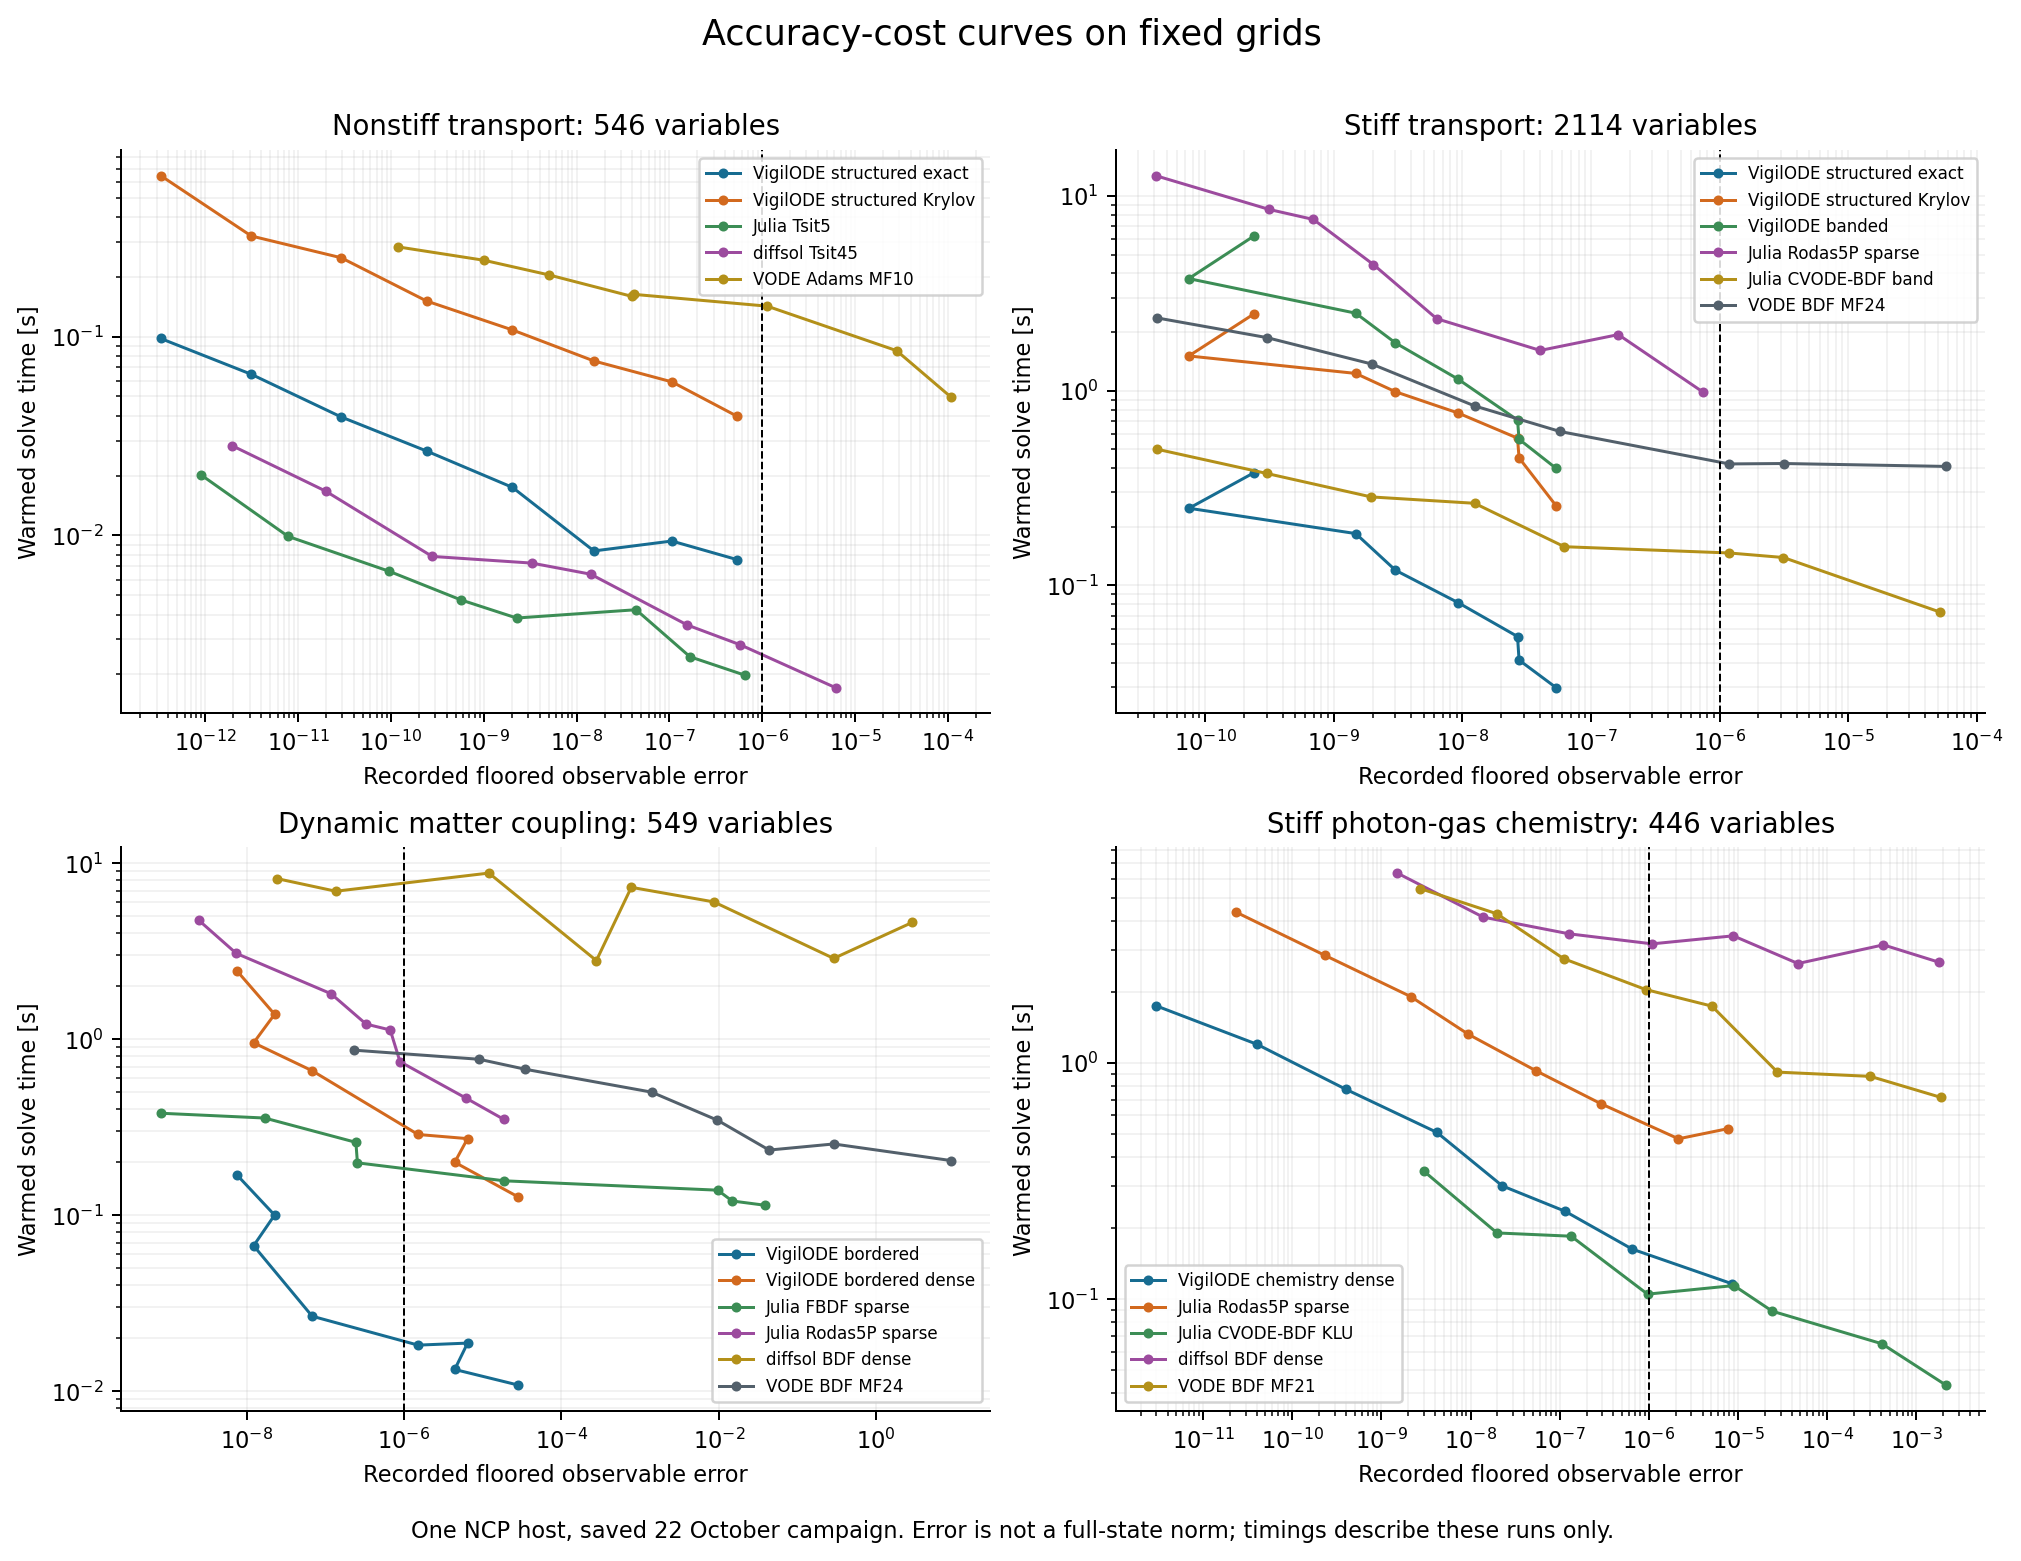
\includegraphics[width=1\textwidth,height=\textheight]{../figures/work_precision.png}
\caption{선택한 문제의 정확도와 계산 비용}
\end{figure}

\textbf{그림 1.} 허용오차별 관측량 오차와 준비 후 내부 적분 시간. 수직
점선은 응용 오차 예산이다. 시간 측정의 구현별 범위 차이가 남아 있으며,
같은 내부 허용오차를 같은 실제 정확도로 해석하지 않는다.

\begin{figure}
\centering
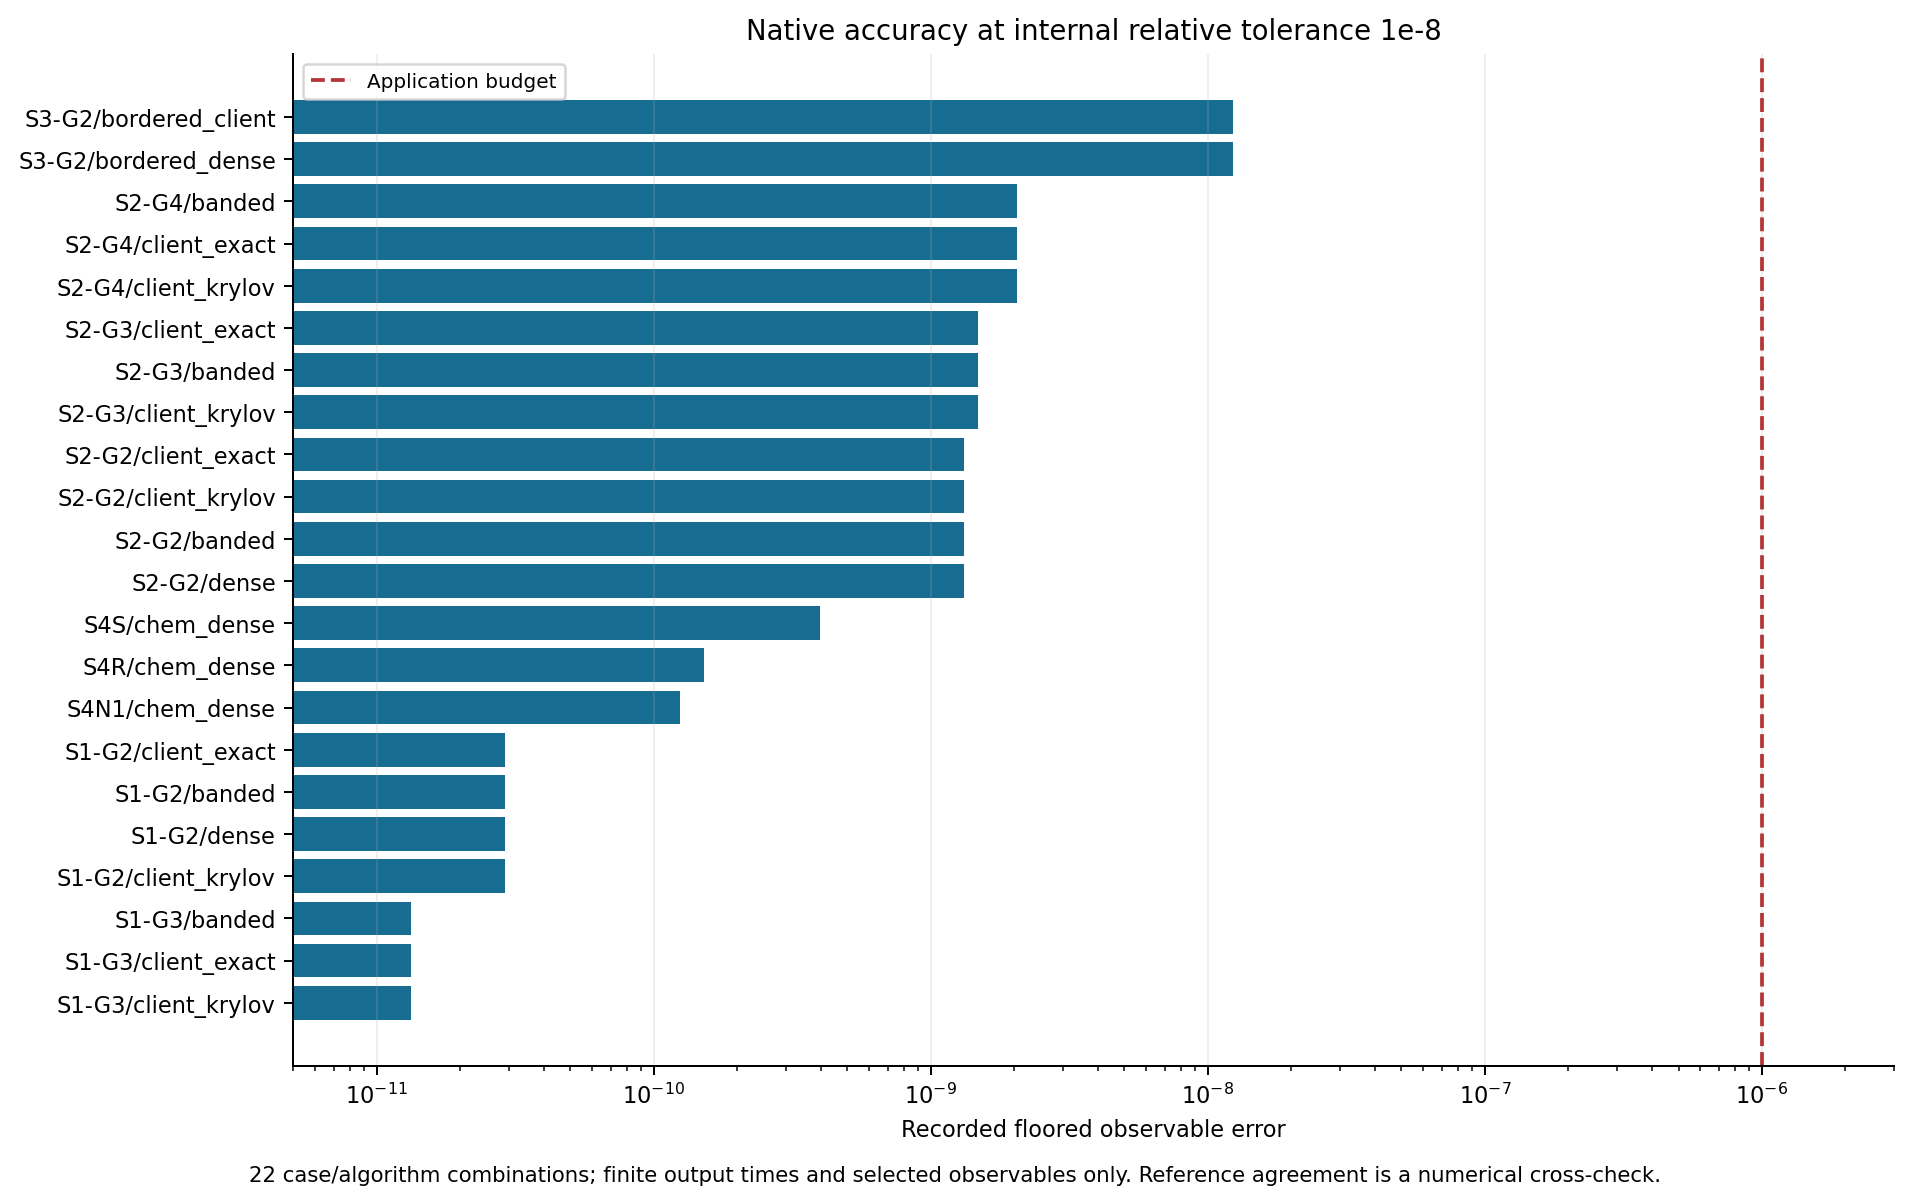
\includegraphics[width=1\textwidth,height=\textheight]{../figures/native_accuracy.png}
\caption{스물두 조합의 관측량 오차}
\end{figure}

\textbf{그림 2.} 내부 상대허용오차 \(10^{-8}\)의 주요 22개 조합. 평가
대상은 지정된 출력 시각과 관측량이며, 전체 분포함수 또는 연속체 해의
오차가 아니다.

\hypertarget{uxac15uxc131-uxc218uxc1a1uxacfc-uxbe44uxac15uxc131-uxc218uxc1a1uxc740-uxb2e4uxb978-uxacb0uxb860uxc744-uxc900uxb2e4}{%
\subsection{강성 수송과 비강성 수송은 다른 결론을
준다}\label{uxac15uxc131-uxc218uxc1a1uxacfc-uxbe44uxac15uxc131-uxc218uxc1a1uxc740-uxb2e4uxb978-uxacb0uxb860uxc744-uxc900uxb2e4}}

단방향 강성 수송에서 군별 정확 풀이의 비용은 격자 크기에 따라 완만하게
증가하였다. 8,322개 상태의 수송에서 게시된 허용오차 선택 실행 시간은
구조 직접 풀이 약 0.0741초, 구조 반복 풀이 약 1.19초, 일반 대역 풀이 약
6.82초이다. 이 값은 한 번의 설정 선택 측정이며, 교차 반복의 시간 비와
섞어 사용하지 않는다. 같은 공간 연산자에서도 선형대수 표현의 차이가 전체
비용을 크게 바꿀 수 있음을 보여준다.

교차 반복에서는 가장 큰 강성 수송 격자에서 Julia 경유 CVODE 대역 해법의
시간이 VigilODE 구조 직접 풀이의 약 15.9배였고, 관측 범위는 약
14.9--17.3배였다. VODE 대역 해법의 비는 약 32.7배, 범위는
30.4--34.9배였다. 이 결과는 해당 물리 구조를 직접 사용한 실행과 범용
대역 해법의 비교이다. 다른 구조나 다른 호스트에서도 같은 비가 유지된다는
결론을 주지 않는다.

반대로 비강성 수송의 2,114개 상태에서는 Julia Tsit5의 시간이 VigilODE의
약 0.222배, diffsol Tsit45는 약 0.278배였다. 강성 억제가 필요하지 않은
구간에서는 여덟 번의 음적 단계 풀이가 불필요한 비용이 될 수 있다. 따라서
범용 사용성을 높이려면 비강성 감지와 명시적 방법의 선택을 실제 오차 조건
아래 평가하는 것이 우선이다.

\begin{figure}
\centering
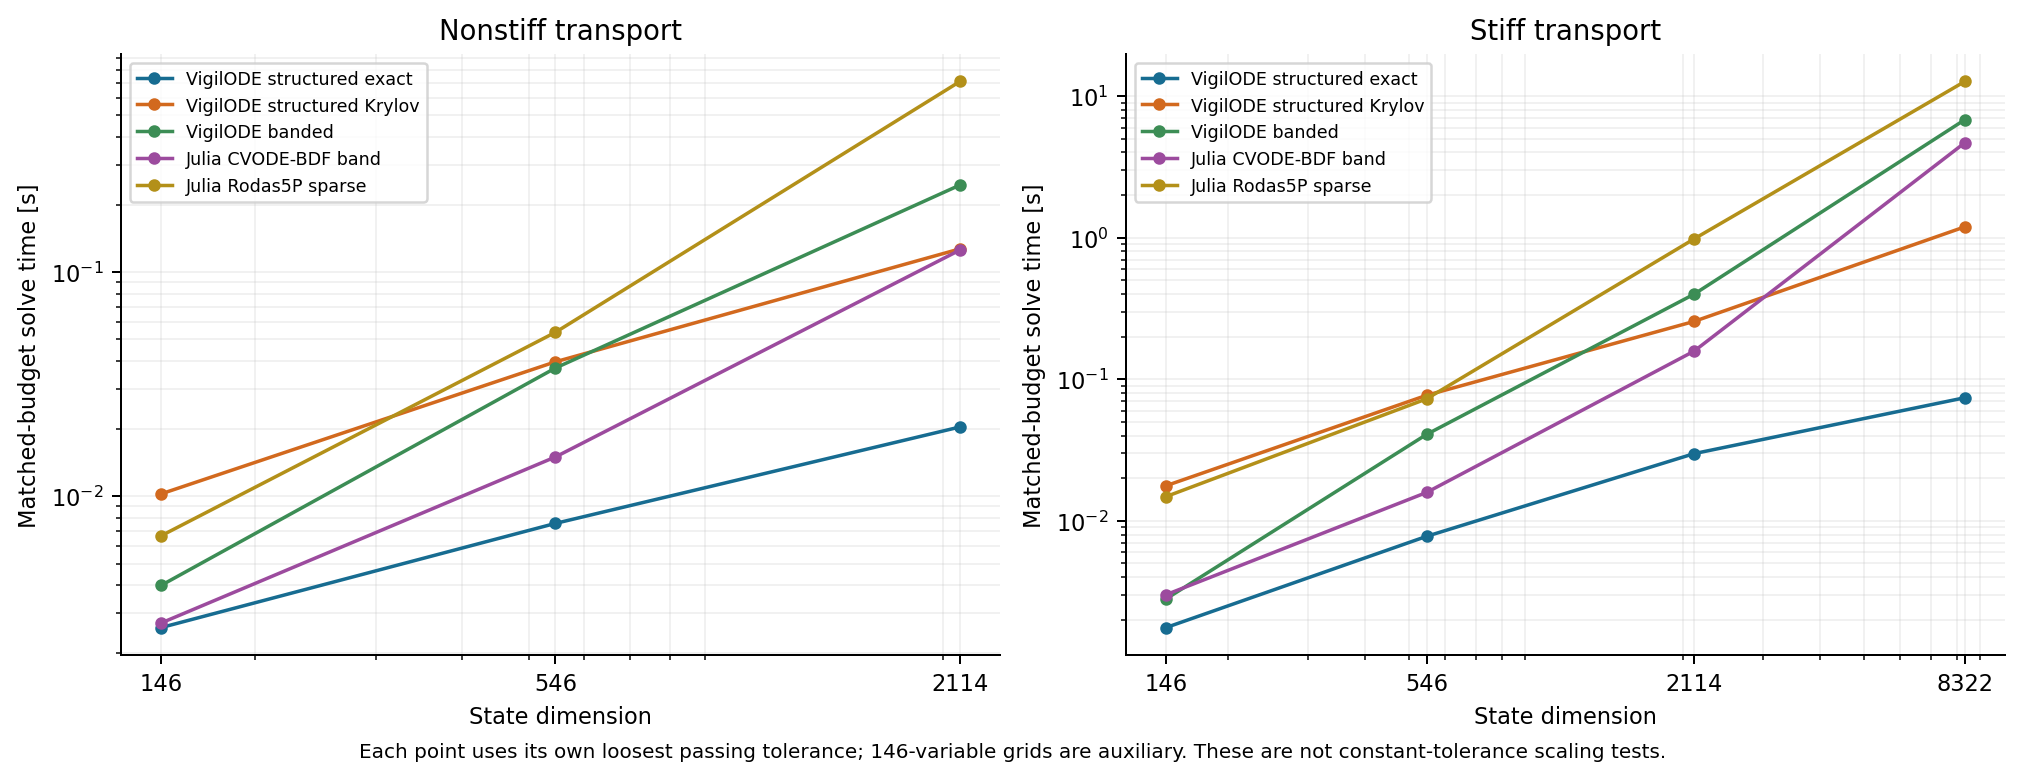
\includegraphics[width=1\textwidth,height=\textheight]{../figures/matched_grid_scaling.png}
\caption{격자 크기에 따른 예산 충족 계산 비용}
\end{figure}

\textbf{그림 3.} 각 격자에서 응용 예산을 만족한 가장 느슨한 허용오차의
시간. 격자마다 허용오차와 단계 수가 다를 수 있으므로 기울기 자체를 점근
복잡도의 측정으로 사용하지 않는다. 가장 느슨한 시험값 \(10^{-3}\)에서
이미 만족한 경우 더 느슨한 설정의 최소 비용은 관측되지 않았다.

\hypertarget{uxacbduxacc4-uxacb0uxd569uxacfc-uxbc18uxc751uxacc4}{%
\subsection{경계 결합과
반응계}\label{uxacbduxacc4-uxacb0uxd569uxacfc-uxbc18uxc751uxacc4}}

광자와 세 물질·기하 변수가 결합된 549차원 문제에서 구조 경계 풀이와 조밀
풀이의 선택 설정 시간은 각각 약 0.0267초와 0.662초였다. 교차 반복에서
Julia FBDF 희소 해법과의 시간 비는 약 5.61, 관측 범위는 약
5.58--5.66이었다. 작은 경계의 Schur 소거가 전체 조밀 분해를 대체할 수
있다는 복잡도 분석과 방향이 일치한다.

446차원 비강성 반응 문제에서는 Julia Tsit5와 diffsol Tsit45가 각각
VigilODE 조밀 해법의 약 0.0496배와 0.113배의 시간을 사용하였다. 강성
반응에서는 결론이 더 혼합되어 있다. 한 강성 경우 Julia 경유 CVODE KLU의
시간이 VigilODE의 약 0.891배였고, 재결합 경우에는 약 1.26배였다. 따라서
반응계에서 모든 대안을 압도하는 하나의 해법이 확인된 것은 아니다. 우선
개선 대상은 비강성 구간의 방법 선택과 강성 반응 Jacobian의 구조화이다.

\begin{figure}
\centering
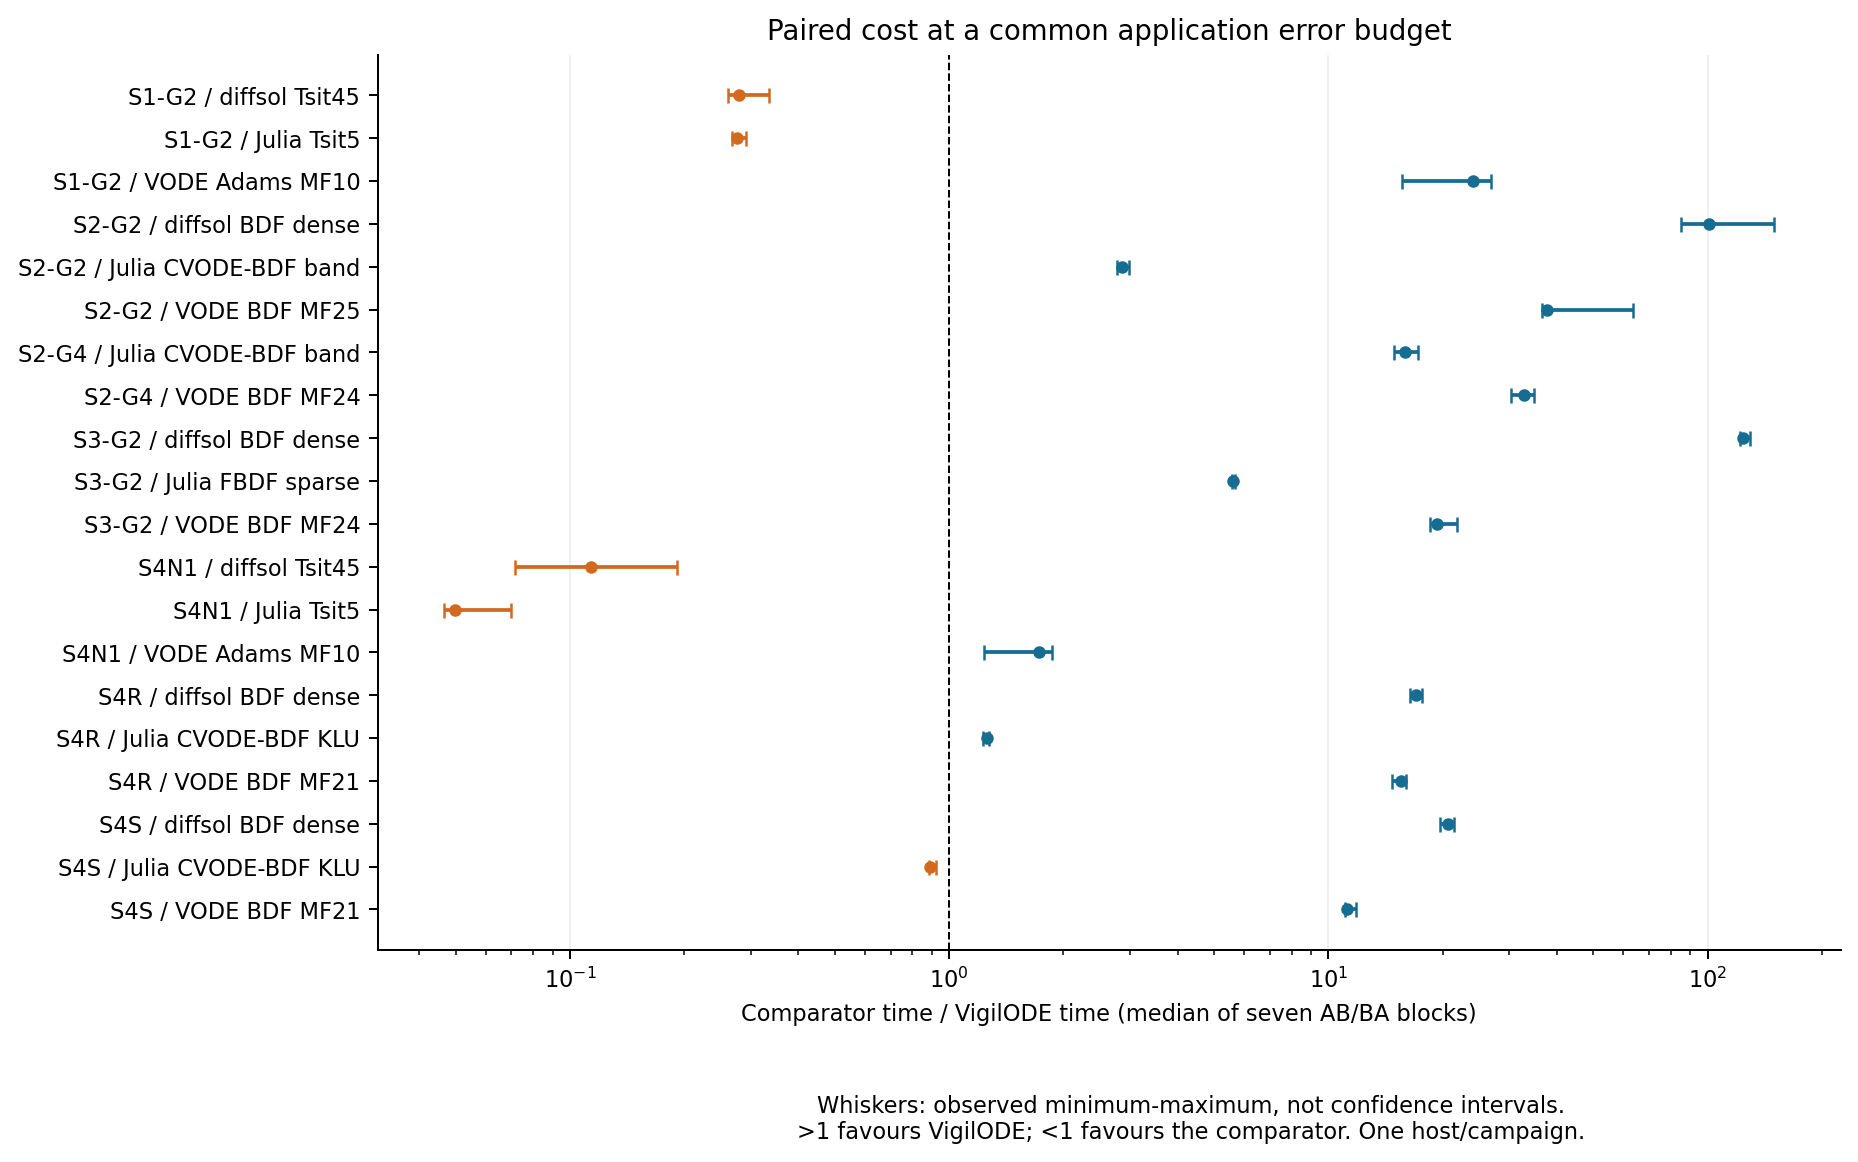
\includegraphics[width=1\textwidth,height=\textheight]{../figures/paired_cost_ratios.png}
\caption{교차 순서 확인 실행의 계산 시간 비}
\end{figure}

\textbf{그림 4.} 비교 방법의 시간/VigilODE 시간의 7개 확인 블록 중앙값과
관측 최솟값--최댓값. 1보다 크면 해당 실행에서 VigilODE가 빨랐다. 선분은
신뢰구간이 아니며 두 방법의 실제 오차가 같다는 의미도 아니다. Julia 경유
CVODE는 SUNDIALS 구현으로 표시하였다.

\hypertarget{uxacfcuxac70-uxc9c4uxb3d9-uxc2dcuxd5d8uxacfc-uxd604uxc7ac-uxacb0uxacfcuxc758-uxad00uxacc4}{%
\subsection{과거 진동 시험과 현재 결과의
관계}\label{uxacfcuxac70-uxc9c4uxb3d9-uxc2dcuxd5d8uxacfc-uxd604uxc7ac-uxacb0uxacfcuxc758-uxad00uxacc4}}

이전 회전 문제의 재검토에서는 낮은 내부 허용오차가 자동으로 원하는 전역
위상 정확도를 주지 않는다는 점이 확인되었다. 게시된 과거 측정 140개 중
응용 기준을 만족한 항목은 7개이며, 모두 더 엄격한 설정에 해당한다.
정확한 전역 위상 오차와 진폭 오차를 별도로 기록해야 한다. 이 사례는 최신
광자 수송 결과를 무효로 만들지 않지만, 수송 관측량의 성공만으로 빠른
진동과 장시간 위상 보존까지 범용성을 확장할 수 없음을 보여준다.

이전 자료의 원시 프로세스 벽시계 시간과 다른 방법의 준비 후 적분 시간을
같은 축에서 비교한 문제도 수정되어야 한다. 현재 연구보고서는 과거의
그러한 그림을 속도 증거로 재사용하지 않는다. 동일한 시간 측정 범위를
갖는 자료만 같은 비교로 해석한다.

\hypertarget{uxd574uxc11duxc801-uxc2a4uxd150uxc2e4uxc758-uxbcc4uxb3c4-uxcd5cuxc801uxd654-uxacb0uxacfc}{%
\subsection{해석적 스텐실의 별도 최적화
결과}\label{uxd574uxc11duxc801-uxc2a4uxd150uxc2e4uxc758-uxbcc4uxb3c4-uxcd5cuxc801uxd654-uxacb0uxacfc}}

별도 결과 브랜치에 게시된 10월 21일의 128차원 주기적 열방정식 실험은
Jacobian 구성에서의 불필요한 우변 평가를 제거한 효과를 보여준다. 기저
벡터별 평가로 Jacobian을 구성하는 대신 해석적 스텐실을 직접 채우면, 전체
우변 평가가 5,712회에서 336회로 줄었다. 게시된 1,046개 실행의 출력
궤적은 동일하였다. 이는 전체 단계 수나 수락 기준을 바꾸지 않고 계산을
제거한 사례이다.

16개 코어에 배치한 확인 블록 480개에서 내부 시간 중앙값은
14.527밀리초에서 8.509밀리초로 감소하였다. 별도 단일 코어 확인 블록
9개를 포함하면 확인 쌍은 489개이다. 그림의 시간 집계는 480개 병행 확인
블록을 사용한다. 이 실험의 소스는
\texttt{5fd6e459a3f67cee90e002821b9b4b740c47475b}이며, 최신 복사·물질
문제 전체의 속도 결과로 전용하지 않는다. 해석적 Jacobian 경로에서도 조밀
저장의 초기화와 조밀 LU 비용이 자동으로 사라지는 것은 아니다.

\begin{figure}
\centering
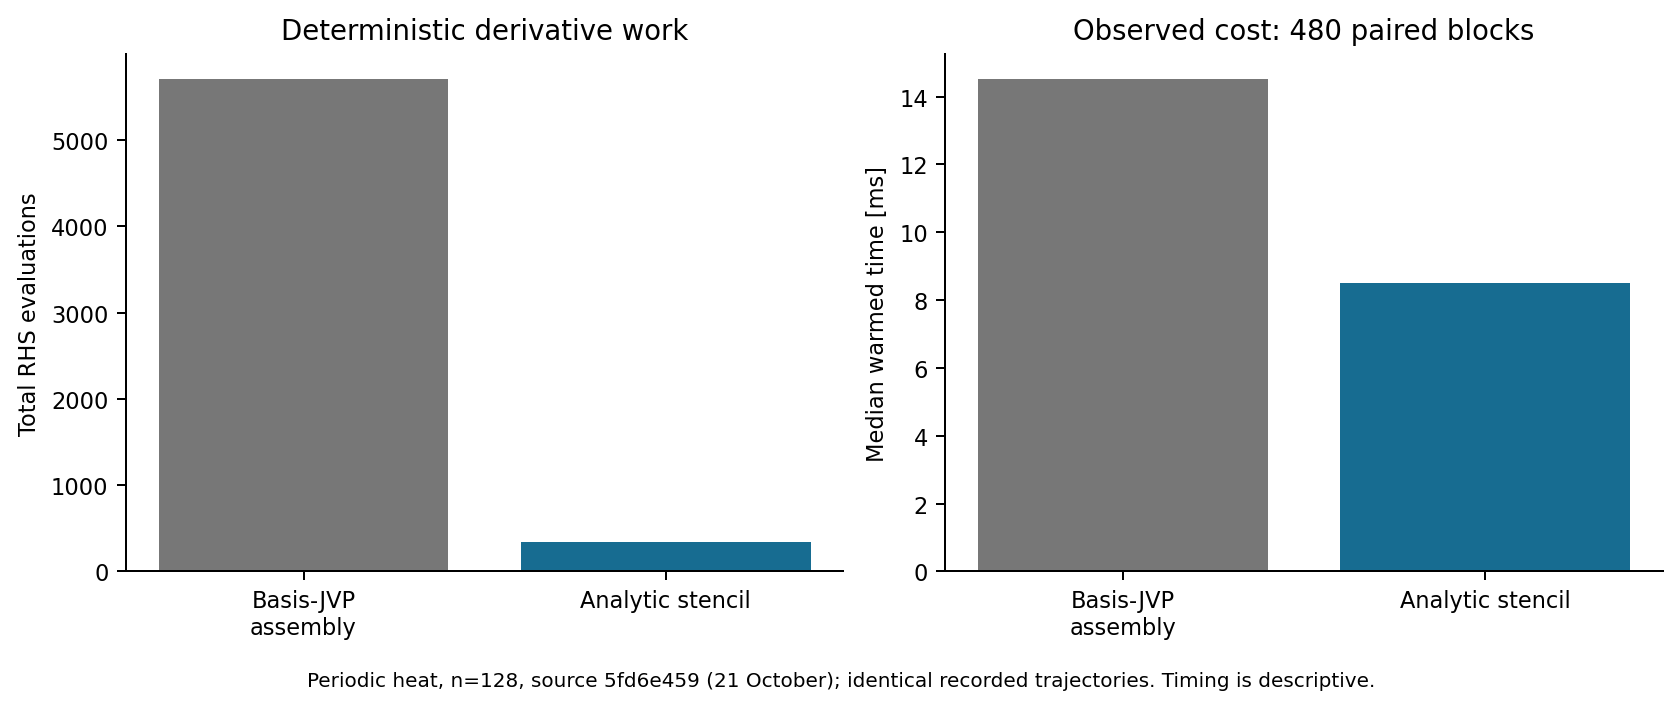
\includegraphics[width=1\textwidth,height=\textheight]{../figures/stencil_work_reduction.png}
\caption{해석적 스텐실의 계산량과 실행 시간 감소}
\end{figure}

\textbf{그림 5.} 별도 열방정식 실험의 우변 평가 수와 내부 시간. 계산량
감소는 구현 변경으로 확인한 사실이며 실행 시간 비는 해당 호스트와 실행
구성에서의 관측이다.

\hypertarget{uxac8cuxc2dc-uxc790uxb8ccuxb85c-uxd655uxc778uxd560-uxc218-uxc788uxb294-uxbc94uxc704}{%
\subsection{게시 자료로 확인할 수 있는
범위}\label{uxac8cuxc2dc-uxc790uxb8ccuxb85c-uxd655uxc778uxd560-uxc218-uxc788uxb294-uxbc94uxc704}}

저장소에 게시된 허용오차 사다리와 교차 반복 JSONL로 설정 선택, 항목 수
및 시간 비를 다시 계산할 수 있다. 그러나 최신 실행의 모든 요청·전체 상태
궤적·기준 상태는 저장소에 포함되어 있지 않고 큰 원자료 압축파일의 해시만
제공되어 있다. 따라서 외부 독자는 현재 게시 자료만으로 관측량 오차를
전체 상태에서 처음부터 재계산할 수 없다.

이는 수치 결과가 틀렸다는 증거가 아니라 검증 가능한 범위의 제한이다.
외부 심사를 완결하려면 두 원자료 압축파일 또는 그 내용과 동등한 축소
재현 패키지를 접근 가능한 위치에 게시해야 한다. 각 결과의 원래 입력,
출력 시각, 상태 배열, 기준 배열, 척도와 소프트웨어 버전을 함께 제공하는
것이 최소 요건이다.

\hypertarget{uxcf54uxb4dc-uxac10uxc0acuxc5d0uxc11c-uxb4dcuxb7ecuxb09c-uxbb38uxc81cuxc640-uxac1cuxc120}{%
\section{코드 감사에서 드러난 문제와
개선}\label{uxcf54uxb4dc-uxac10uxc0acuxc5d0uxc11c-uxb4dcuxb7ecuxb09c-uxbb38uxc81cuxc640-uxac1cuxc120}}

이번 검토에서 구조 단계 해법의 입력 길이를 검사하지 않은 호출 경로,
실패한 인수분해 뒤 과거 인수를 사용 가능한 상태로 남기는 경로, 그리고
반복 단계 풀이를 이중으로 세는 작업량 기록이 확인되었다. 첫 문제는
잘못된 슬라이스 길이가 명시적 오류 대신 패닉으로 이어질 수 있다. 둘째는
실패 후 재사용의 의미를 훼손한다. 셋째는 수치 해 자체보다 해법 간 작업량
비교의 정확성을 훼손한다. 수정은 입력 검사를 계산 전에 수행하고,
재분해를 시작할 때 이전 상태를 무효화하며, 외부 적분기와 내부 GMRES가
소유하는 계수를 분리하는 방향으로 이루어졌다. 세 변경의 표적 회귀 결과는
함께 제공되는 검증 기록에 대응한다.

관측량 평가에서도 기준 복사 에너지의 정의역을 명시적으로 검사해야 한다.
소멸 가중치를 계산할 때 음의 기준 에너지가 들어가면 음의 가중치가 오차를
작게 보이게 할 수 있기 때문이다. 이를 정상적인 정확도 성공으로 취급하지
않는 입력 검사를 추가하였다. 과거에 저장된 실험 결과를 새 입력 검사로
무단 덮어쓰지 않고, 이후 평가에 적용할 계약과 회귀 사례를 남긴다.

이번에 추가한 원래 차원의 저랭크 경계 전처리는 기존의 응용 전용 풀이를
범용 선형대수 구성으로 확장한다. 용량과 차원, 유한 입력, 특이 작은 행렬,
실패 뒤 인수 무효화와 반복 적용의 작업공간을 명시한다. 이 구성은 특정
수송 문제의 빠른 풀이를 대체하기 위해 무조건 호출하는 기본값이 아니다.
실제 추가 저랭크 결합이 있는 응용 문제에서 전체 비용과 잔차를 평가한 뒤
선택해야 한다.

별도의 VigilODE 개발에서 이미 해결된 과거 문제를 미해결 목록에 다시
올리지 않았다. 범용 공개 인터페이스, 벡터 절대허용오차, 내부 출력 오차
제어, 실패 통계와 사건 자료의 개선은 현재 소스에 포함되어 있다. 현재
문제는 이런 기능의 부재보다는 지원 조합의 명확성, 실제 사용자 경로에서의
통합 정도, 그리고 검증된 범위의 확장이다.

\hypertarget{uxc774uxbc88-uxc218uxc815uxc758-uxc2e4uxc81c-uxac80uxc99d}{%
\subsection{이번 수정의 실제
검증}\label{uxc774uxbc88-uxc218uxc815uxc758-uxc2e4uxc81c-uxac80uxc99d}}

이번 변경에 대해 수행한 표적 검증은 아래와 같다. 실패를 먼저 재현한 세
회귀 사례는 수정 후 정상 통과하였고, 과거의 변경 없는 전체 시험 묶음을
다시 실행한 수로 합산하지 않았다.

\begin{longtable}[]{@{}
  >{\raggedright\arraybackslash}p{(\columnwidth - 4\tabcolsep) * \real{0.3000}}
  >{\raggedleft\arraybackslash}p{(\columnwidth - 4\tabcolsep) * \real{0.4000}}
  >{\raggedright\arraybackslash}p{(\columnwidth - 4\tabcolsep) * \real{0.3000}}@{}}
\toprule\noalign{}
\begin{minipage}[b]{\linewidth}\raggedright
검증 대상
\end{minipage} & \begin{minipage}[b]{\linewidth}\raggedleft
실제 실행
\end{minipage} & \begin{minipage}[b]{\linewidth}\raggedright
확인한 의미
\end{minipage} \\
\midrule\noalign{}
\endhead
\bottomrule\noalign{}
\endlastfoot
사용자 정의 단계 해법 & Rust 시험 11개 통과 & 새 회귀 3개와 기존 관련
시험 8개; 입력 길이·실패 후 인수 무효화·단계 풀이 계수 \\
원래 차원 저랭크 전처리 & Rust 시험 8개 통과 & 계약 6개, 성공 경로 할당
1개, 실제 GMRES 연결 1개 \\
관측량 입력 정의역 & Python 시험 3개 통과 & 잘못된 기준 입력이 작은
오차로 처리되지 않음 \\
아핀 복원 오차 노름 & 유한 예 10개와 부정 입력 대조 5개 통과 & 고정밀
Decimal 기준과의 비교 및 출력 보존 \\
\end{longtable}

이 검증은 현재 수정 코드의 의미를 확인한다. 최신 NCP의 긴 실행은 수치
소스
\href{https://github.com/cosmosapjw-quantum/vigilode/commit/2064366ea39ef35a9eae7966b4b5b2424a46124c}{\texttt{2064366e}}의
실행이고, 본 감사의 코드 변경을 포함한 새 NCP 실행은 수행하지 않았다.
따라서 원래 측정의 실행 시간과 정확도를 새 구현의 실측값으로 다시
표기하지 않는다. 새 저랭크 구성의 핵심 등식·복잡도와 표적 시험은
확보했으며, 실제 응용 문제에 연결한 전체 적분 및 목표 호스트 성능은 후속
검증에 남는다.

\hypertarget{uxc6b4uxc601-uxc801uxd569uxc131-uxd310uxc815uxacfc-uxb2e4uxc74c-uxac1cuxbc1c-uxb2e8uxacc4}{%
\section{운영 적합성 판정과 다음 개발
단계}\label{uxc6b4uxc601-uxc801uxd569uxc131-uxd310uxc815uxacfc-uxb2e4uxc74c-uxac1cuxbc1c-uxb2e8uxacc4}}

\hypertarget{uxd604uxc7ac-uxc0acuxc6a9uxd560-uxc218-uxc788uxb294-uxbc94uxc704}{%
\subsection{현재 사용할 수 있는
범위}\label{uxd604uxc7ac-uxc0acuxc6a9uxd560-uxc218-uxc788uxb294-uxbc94uxc704}}

고정된 물리 모형과 격자, 명시된 허용오차 및 기준해를 가진 연구
계산에서는 현재 구현을 유용하게 사용할 수 있다. 특히 단방향 에너지
이류와 냉각된 비편광 Thomson 산란을 갖는 축대칭 수송은 선형 계산량의
직접 구성을 갖추고 있으며, 최신 실험은 그 정확도와 비용상의 장점을
뒷받침한다. 다만 이 응용 해법은 일반 목적의 모든 입력을 자동으로
처리하는 해법과 구분하여 배포해야 한다.

범용 production solver로서의 무조건적 사용을 현재 자료만으로 승인하기는
어렵다. 필요한 것은 새로운 이름의 성공 기준을 추가하는 일이 아니라, 실제
사용자가 기대하는 입력·출력·실패·정확도의 범위를 완결하는 일이다. 아래
작업은 그 공백에 직접 대응한다.

\hypertarget{uxc815uxd655uxb3c4-uxac1cuxc120uxc758-uxc6b0uxc120uxc21cuxc704}{%
\subsection{정확도 개선의
우선순위}\label{uxc815uxd655uxb3c4-uxac1cuxc120uxc758-uxc6b0uxc120uxc21cuxc704}}

\textbf{첫째, 전체 상태와 관측량을 함께 검증한다.} 최신 원자료를
공개하고 각 셀의 가중 오차, 최소 분포값, 위상·모멘트 오차 및 보존량을
같은 출력 시각에서 계산해야 한다. 관측량 예산은 그대로 유지하고, 전체
상태 검사를 추가한다. 기존 예산을 더 느슨하게 바꾸어 통과시키는 방식은
적절하지 않다.

\textbf{둘째, 시간과 공간의 수렴을 분리한다.} 고정 격자에서 시간
허용오차를 줄이는 시험, 매우 엄격한 시간 설정에서 격자를 줄이는 시험, 두
오차를 함께 줄이는 시험을 구분한다. 비매끄러운 이온화 문턱과 재격자화
시점은 별도 패널에 표시한다. 선형계 잔차가 시간 오차 추정과 같은 규모가
되면 더 정확한 단계 풀이가 필요하다.

\textbf{셋째, 축소 좌표의 오차 제어를 적분기에 연결한다.} 아핀 노름
커널을 호출하는 안전한 경계와 실패 처리를 만들고, 전체 표현과 축소
표현을 같은 물리 초기값·척도로 비교한다. 수락 단계의 개수가 꼭 같아야 할
필요는 없으나, 두 표현이 같은 물리적 오차 기준을 적용한다는
수학적·수치적 대응은 필요하다.

\textbf{넷째, 재격자화의 누적 예산을 제어한다.} 한 번의 보존 오차뿐
아니라 재구성 결함의 누적값을 기록하고, 재격자화 빈도와 격자 해상도를
함께 변경한다. 양성 보정이 필요하면 그 보정이 바꾼 수·에너지·고차
모멘트를 기록한다. 제한자 또는 보정의 효과를 시간 적분기의 차수로 숨기지
않는다.

\hypertarget{uxc18duxb3c4-uxac1cuxc120uxc758-uxc6b0uxc120uxc21cuxc704}{%
\subsection{속도 개선의
우선순위}\label{uxc18duxb3c4-uxac1cuxc120uxc758-uxc6b0uxc120uxc21cuxc704}}

\textbf{구조 직접 풀이를 먼저 선택한다.} 단방향 에너지 이동에서 이미
정확한 선형 비용 풀이가 있다면 GMRES를 반드시 거칠 이유가 없다. 구조
검사와 실패 시 대체 경로를 명시하고, 반복 해법은 혼합 방향이나 더 복잡한
결합에 집중한다. 최신 측정에서도 반복 해법의 일반성이 정확 직접 풀이보다
낮은 비용을 보장하지 않았다.

\textbf{강성 반응망의 작은 경계를 분리한다.} 광자 블록과 소수의 물질
변수를 나누고, 새 저랭크 구성이나 물질 Schur 소거로 전체 조밀 분해를
줄인다. 먼저 준비·적용·반복·우변·출력의 개별 비용을 측정하여 실제 병목을
확인한다. 작은 행렬을 구성하는 비용이 우변을 지배하면 구조화의 이득이
작아질 수 있다.

\textbf{비강성 구간의 방법 선택을 추가한다.} 최신 결과에서 명시적 방법이
더 빠른 구간을 확인했으므로, 강성 검출과 방법 전환을 별도 후보로 개발할
근거가 있다. 전환 조건, 전환 시 상태·오차 이력 및 사건·출력의 연속성을
고정한 뒤, 한 가지 방법만 유지한 대조군과 비교한다.

\textbf{반복 자료의 재사용을 변화량에 연결한다.} 행렬·단계
크기·격자·물리 계수가 바뀔 때 전처리나 반복 부분공간을 그대로 재사용할
수 있는 조건을 기록한다. 수렴 정리의 \(\|\Delta\mathcal MP^{-1}\|\) 또는
계산 가능한 보수적 대체량을 이용하여 재구성 시점을 정할 수 있다. 단순
재사용 횟수와 실제 오차를 혼동하지 않는다.

\textbf{재격자화 할당을 구간 밖 비용으로 최적화한다.} 현재의 구간 내부
무할당 장점을 유지하면서 최대 용량의 모델·단계·선형계·출력 버퍼를
공유하는 인터페이스를 설계한다. 단일 커널의 무할당 시험에 더해
재격자화가 실제로 발생하는 전체 실행의 할당과 최대 메모리를 측정한다.

\hypertarget{uxb2e4uxd56duxc2dduxacfc-uxc2dcuxac04-uxbcd1uxb82cuxd654uxc758-uxc704uxce58}{%
\subsection{다항식과 시간 병렬화의
위치}\label{uxb2e4uxd56duxc2dduxacfc-uxc2dcuxac04-uxbcd1uxb82cuxd654uxc758-uxc704uxce58}}

Laguerre·Chebyshev·Leja 다항식이나 행렬함수 작용은 Krylov 부분공간을
형성하는 비용을 줄일 가능성이 있다. 다만 이러한 후보는 동일한 함수 작용,
스펙트럼 또는 수치범위 정보, 비정규성, 다항식 절단오차와 반올림 오차를
함께 다루어야 한다. 어떤 기저가 모든 문제에 우세하다는 순서는 정해져
있지 않다. 감쇠가 지배하는 스펙트럼에는 Laguerre 표현이 유용할 수 있고,
실수 구간에 가까운 연산자에는 Chebyshev 또는 Leja 구조가 적합할 수 있다.
후보별 전체 비용에는 계수·절점 준비와 경계 추정의 비용도 포함된다.

Homotopy와 시간 병렬화는 순차 시간 진행을 더 짧은 종속 사슬로 바꾸려는
다른 방향이다. 하나의 시간 구간에서 얻은 끝점을 다음 구간의 정확한
초기값으로 사용하는 문제를 단순 병렬 호출로 대체할 수는 없다. 구간별
예측과 접합 결함을 명시하고, 전역 경계 결함에 대한 수축 조건 또는 보정의
수렴을 확보해야 한다. 병렬 구간 수가 증가하면서 필요한 보정 반복도
증가하면 총 가속은 사라질 수 있다. 따라서 먼저 작은 비선형 문제에서 접합
결함과 전역 오차를 동일한 기준으로 측정한 뒤, 실제 물리 문제의 다중
시간척도에 확장하는 것이 타당하다. 현재 최신 수송 벤치마크는 이 후보들의
속도 증거가 아니다.

\hypertarget{uxacb0uxb860}{%
\section{결론}\label{uxacb0uxb860}}

VigilODE의 최근 진전은 고차 시간 적분기를 구현했다는 사실을 넘어선다.
범용 인터페이스의 오류 처리와 오차 의미를 정리하고, 광자 수송의 국소
결합과 저랭크 산란을 실제 단계 선형계에 연결했으며, 수락 단계 사이의
보존형 재격자화를 작동하는 코드 경로로 만들었다. 단방향 수송의 선형
복잡도 직접 풀이와 작은 물질 경계의 소거는 조건이 분명한 계산량
감소이다. 원래 차원의 저랭크 보정과 아핀 복원 오차 노름은 이 구조를 더
넓은 응용 문제에 적용할 수 있는 다음 연결이다.

측정 결과는 응용에 따라 방법을 선택해야 한다는 결론을 지지한다. 강성
수송에서는 구조 직접 풀이가 유리하고, 비강성 수송·반응에서는 명시적
대안이 유리하며, 강성 반응에서는 희소 BDF와의 경쟁이 남아 있다. 현재의
관측량 정확도는 충분히 고무적이지만 전체 상태와 연속체 정확도, 실제
BASS/rei 결합 및 모든 기능 조합의 운영 안정성을 대신하지 않는다.

따라서 다음 개발의 중심은 증명할 수 있는 구조를 실제 경로에 연결하고, 그
경로의 전체 물리 오차와 전체 비용을 함께 측정하는 데 두어야 한다. 원자료
공개, 축소 노름의 수락 경로 연결, 혼합 방향 전처리의 정량적 수렴 평가,
공간·시간·재매핑 오차의 분리 검증을 완료하면 현재의 제한된 연구 사용을
더 넓은 운영 범위로 확장할 수 있다.

\hypertarget{uxbd80uxb85d-a.-uxc678uxbd80-uxc7acuxd604uxc5d0-uxd544uxc694uxd55c-uxc790uxb8cc}{%
\section*{부록 A. 외부 재현에 필요한
자료}\label{uxbd80uxb85d-a.-uxc678uxbd80-uxc7acuxd604uxc5d0-uxd544uxc694uxd55c-uxc790uxb8cc}}
\addcontentsline{toc}{section}{부록 A. 외부 재현에 필요한 자료}

재현자는 원래 수치 소스와 본 감사의 수정 소스를 구분해야 한다. 최신 NCP
측정은 수정 전 소스를 실행한 결과이며, 이번에 추가한 일반 저랭크
전처리의 속도 측정으로 읽으면 안 된다. 저장소에는 알고리즘 소스, 고정
계수 스냅샷, 측정 계획·집계·교차 반복 자료, 본 보고서의 그림 생성 코드와
이번 수정의 회귀 결과가 함께 제공된다.

최소 재현 단위는 소스 commit, 의존성 잠금 파일, 컴파일러 및 플래그,
하드웨어·스레드 배치, 문제 입력, 출력 시각, 기준해, 오차 정의, 정상·실패
원자료, 그리고 집계 스크립트이다. 파일의 해시는 내용의 동일성을
확인하지만 물리·수치적 타당성을 대신하지 않는다. 큰 원자료 압축파일을
별도 위치에 둘 때도 이 항목들이 함께 복원되어야 한다.

\hypertarget{uxbd80uxb85d-b.-uxc2dduxacfc-uxad6cuxd604uxc758-uxb300uxc751}{%
\section*{부록 B. 식과 구현의
대응}\label{uxbd80uxb85d-b.-uxc2dduxacfc-uxad6cuxd604uxc758-uxb300uxc751}}
\addcontentsline{toc}{section}{부록 B. 식과 구현의 대응}

\begin{longtable}[]{@{}
  >{\raggedright\arraybackslash}p{(\columnwidth - 2\tabcolsep) * \real{0.5000}}
  >{\raggedright\arraybackslash}p{(\columnwidth - 2\tabcolsep) * \real{0.5000}}@{}}
\toprule\noalign{}
\begin{minipage}[b]{\linewidth}\raggedright
본문 구성
\end{minipage} & \begin{minipage}[b]{\linewidth}\raggedright
주요 소스 위치
\end{minipage} \\
\midrule\noalign{}
\endhead
\bottomrule\noalign{}
\endlastfoot
RODAS5P 계수·변환 & \texttt{crates/rodas5p-core/src/coefficients.rs} \\
여덟 단계 빠른 적분 &
\texttt{crates/rodas5p-integrators/src/rodas5p\_fast.rs} \\
사용자 정의 단계 선형계 &
\texttt{crates/rodas5p-integrators/src/client\_stage.rs} \\
범용 공개 인터페이스 & \texttt{crates/vigilode/src/problem.rs},
\texttt{options.rs}, \texttt{solve.rs} \\
대역·작은 경계 소거 & \texttt{crates/rodas5p-core/src/bordered.rs} \\
원래 차원 저랭크 보정 &
\texttt{crates/rodas5p-core/src/low\_rank\_bordered.rs} \\
보존형 겹침 매핑 &
\texttt{crates/rodas5p-integrators/src/conservative\_remap.rs} \\
축대칭 수송·군별 풀이 &
\texttt{crates/rodas5p-integrators/examples/lrs\_photon\_fv\_support/} \\
전체 구면 수송 &
\texttt{crates/rodas5p-integrators/examples/sphere\_photon\_fv\_support/} \\
아핀 복원 오차 노름 &
\texttt{research/lifted\_error\_norm\_20261022/code/lifted\_error\_norm.c} \\
최근 비교의 오차 평가 &
\texttt{external\_audits/vigilode\_bassrei\_ncp\_c1\_20261022/harness/} \\
\end{longtable}

\hypertarget{uxcc38uxace0uxbb38uxd5cc}{%
\section*{참고문헌}\label{uxcc38uxace0uxbb38uxd5cc}}
\addcontentsline{toc}{section}{참고문헌}

{[}1{]} SciML, \emph{OrdinaryDiffEq.jl: RODAS5P coefficient
implementation}. 본 소스의 저자 계수 참조 commit
\texttt{000230a3e53a445a22c090aff9148430367a0a74},
\texttt{src/tableaus/rosenbrock\_tableaus.jl}.
\url{https://github.com/SciML/OrdinaryDiffEq.jl/blob/000230a3e53a445a22c090aff9148430367a0a74/src/tableaus/rosenbrock_tableaus.jl}.

{[}2{]} J. Lang and J. G. Verwer, ``ROS3P---An Accurate Third-Order
Rosenbrock Solver Designed for Parabolic Problems,'' \emph{BIT Numerical
Mathematics} \textbf{41} (2001), 731--738. 원문:
\url{https://ir.cwi.nl/pub/1102/1102D.pdf}.

{[}3{]} M. F. Murphy, G. H. Golub and A. J. Wathen, ``A note on
preconditioning for indefinite linear systems,'' \emph{SIAM Journal on
Scientific Computing} \textbf{21} (2000), 1969--1972. DOI:
\url{https://doi.org/10.1137/S1064827599355153}.

{[}4{]} B. S. Southworth, A. A. Sivas and S. Rhebergen, ``On
fixed-point, Krylov, and 2×2 block preconditioners for nonsymmetric
problems,'' \emph{SIAM Journal on Matrix Analysis and Applications}
(2020). DOI: \url{https://doi.org/10.1137/19M1298317}. 저자 공개본:
\url{https://arxiv.org/abs/1911.02664}.

{[}5{]} Y. Saad and M. H. Schultz, ``GMRES: A generalized minimal
residual algorithm for solving nonsymmetric linear systems,'' \emph{SIAM
Journal on Scientific and Statistical Computing} \textbf{7} (1986),
856--869. DOI: \url{https://doi.org/10.1137/0907058}.

{[}6{]} VigilODE 개발 저장소, 수치 소스·계수·시험 및 NCP 측정 자료,
2026년 10월 22일 확인.
\url{https://github.com/cosmosapjw-quantum/vigilode}.

{[}7{]} G. Steinebach, ``Construction of Rosenbrock--Wanner method
Rodas5P and numerical benchmarks within the Julia Differential Equations
package,'' \emph{BIT Numerical Mathematics} \textbf{63} (2023), article
27. DOI: \url{https://doi.org/10.1007/s10543-023-00967-x}.

\end{document}
